\setcounter{chapter}{8-1} 

\chapter{Transformers}


In this chapter, we want to focus on processing language. In particular:\\

\begin{definition}
    \vocab{Natural Language Processing} (NLP) is a field of machine learning all about processing, understanding, and using \gren{human language}.
\end{definition}

\begin{itemize}
    \item \miniex Chatbots, language translation, etc.
\end{itemize} 

We'll start by considering a few candidate models for NLP, before moving to the state-of-the-art: \orgg{transformers}.

\subsection{CNNs}

    In the previous chapter, we introduced the notion of a CNN:

    \begin{itemize}
        \item \vocab{Convolutional Neural Networks (CNNs)} view small regions of data, searching for patterns across the image.

        \begin{figure}[H]
            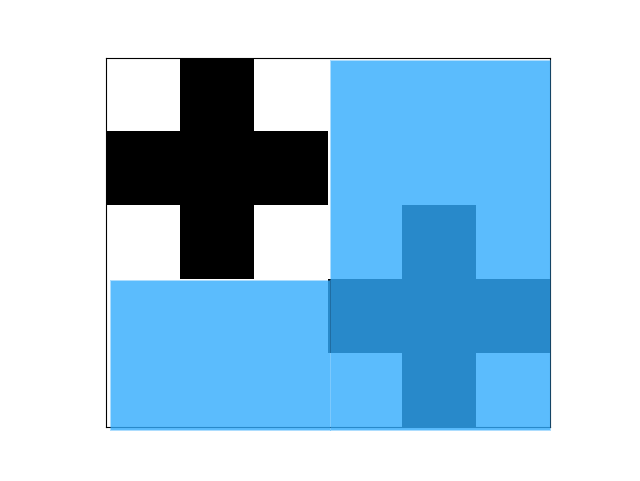
\includegraphics[width=40mm,scale=0.5]{images/convolutional_neural_networks_images/window.png}
            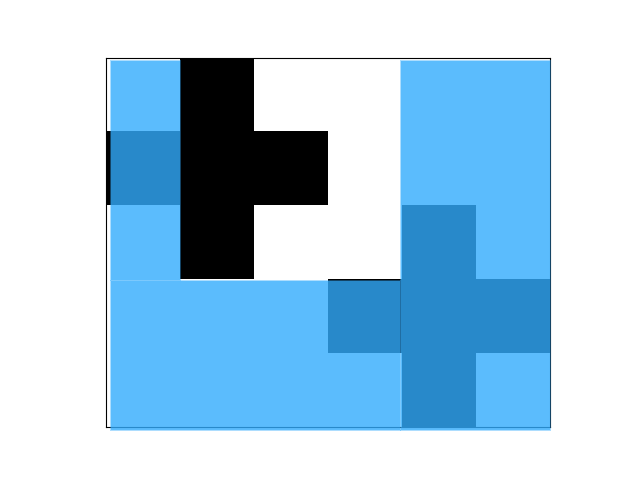
\includegraphics[width=40mm,scale=0.5]{images/convolutional_neural_networks_images/window2.png}
            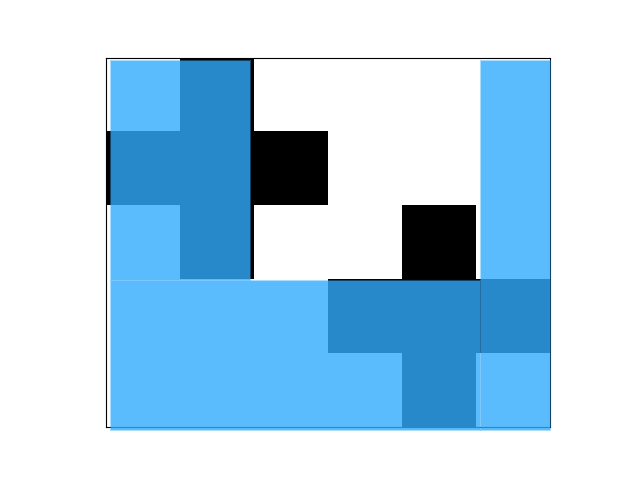
\includegraphics[width=40mm,scale=0.5]{images/convolutional_neural_networks_images/window3.png}
            
            \caption*{In this example, we focus on a 3x3 segment of our data.}
        \end{figure}

        
    \end{itemize}

    This kind of structure is useful for image processing: nearby pixels tend to be related to each other.
        \note{They might form a single line, or a corner, for example.}

    \begin{itemize}
        \item By prioritizing "nearby" information, we can create models that easily find those \textbf{localized} patterns.
        
        \item We called this property \textbf{spatial locality}.
    \end{itemize}

    \begin{concept}
        CNNs are designed to represent \vocab{locality}:

        \begin{itemize}
            \item In a CNN, \purp{nearby} data is used to search for patterns.
        \end{itemize}

        This allows us to use smaller, \orgg{simpler} models:

        \begin{itemize}
            \item Rather than thinking about every possible connection between data, we only connect "nearby" data. Thus, we need \gren{fewer} parameters.
        \end{itemize}
    \end{concept}




\phantom{}

\subsection{The problem with locality}

    This presents one simple weakness, that we've ignored so far:

    \begin{itemize}
        \item If we focus on information that is \textbf{nearby}, we're missing out on information that's \orgg{far away}.

        \item We need a way to encode "distance" of information, that doesn't ignore the "distant" info.\\
    \end{itemize}

    \begin{concept}
        If information is spread over \vocab{long distances}, our CNN model won't capture it.

        \begin{itemize}
            \item If a pattern is \purp{too big} for our CNN filter, we'll have more trouble finding it.
        \end{itemize}
    \end{concept}

    This can become especially problematic for \textbf{language} processing.

    \miniex Consider the following sentence: 

    \begin{itemize}
        \item \redd{The sweater} that I found in the back of my old closet, which I hadn't opened since we moved into the house several years ago, \redd{still fits me perfectly.}
    \end{itemize}

    \phantom{}

    Note that the beginning and the end of this sentence are linked as a single idea: "\blu{The sweater still fits me perfectly}".

    \begin{itemize}
        \item But there's a \purp{huge gap} between these phrases: it might be difficult to connect information over such a wide gap, while \orgg{ignoring} what's in-between. 

        \item This also comes up in longer passages: in a paragraph, the first sentence might create \gren{context} for the last sentence.
           
    \end{itemize}

    \begin{concept}
        In language, words can be \purp{far apart}, while still providing important \gren{context} for the meaning of the text.

        \begin{itemize}
            \item Thus, language processing is difficult for models which focus too much on \vocab{locality}.
        \end{itemize}
    \end{concept}

\phantom{}

\subsection{RNNs}

    One useful observation might be that language tends to be \textit{sequential}: words come in a very particular order.\\

    \begin{concept}
        In \vocab{image processing}, we see many pixels at the same time: the whole image is processed in \purp{parallel}.

        In \vocab{language processing}, we hear/read words one-by-one, in order: the data has a \gren{sequential} structure.
    \end{concept}

    Recurrent Neural Networks (RNNs) are, thus, a \textbf{sequential} model, designed for processing language.

    \begin{figure}[H]
        \centering
        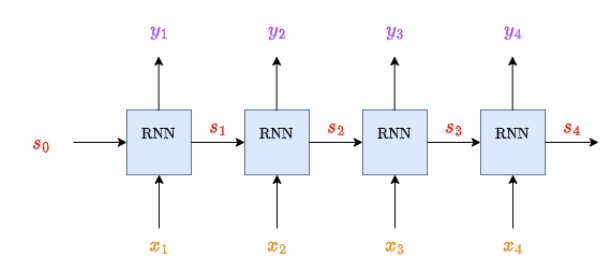
\includegraphics[width=90mm,scale=0.5]{images/transformers_images/rnn_sequential.png}
        \caption*{Each $x_t$ is one word in our sentence: we process the text, one word at a time. After every word, we update our memory ("state" $s_t$). $y_t$ is our output at time $t$.}
    \end{figure}

    By storing information about previous words (using a \gren{state}), our model can "read" each word \purp{in order}, while still remembering earlier parts of the text.

    \begin{itemize}
        \item While a CNN can only observe $k$ consecutive pixels/words in a row, our RNN might be able to contain \textit{some} information about words that are much further back in time.
    \end{itemize}

    How well does this work? RNNs have seen success in the past, but it struggles with \purp{forgetting}: our RNN can only store so much information about words it's seen before.

    \begin{itemize}
        \item As a passage gets longer, our RNN is only paying attention to words it's seen \gren{recently}.
    \end{itemize}

    Moreover, our RNN doesn't have any way to \purp{choose} which words to \orgg{prioritize}: each new word will have to replace some information about older words. 

    \begin{itemize}
        \item So, our RNN naturally prioritizes the most \gren{recent words}.
            \note{The more recent words haven't been replaced yet.}
            
        \item But the most recent word isn't always the most important one, as we saw above (in the sweater example)!\\
    \end{itemize}

    \begin{concept}
        \vocab{RNNs} (Recurrent Neural Networks) tend to struggle with longer bodies of text:

        \begin{itemize}
            \item The \gren{longer} we run our RNN, the less it usually remembers about the \gren{distant} past.
        \end{itemize}

        Moreover, it prioritizes recent words, even when more distant words may be \orgg{more important}.
        
    \end{concept}

    In the end, RNNs have, in most language applications, been replaced by transformers: a different model for language processing.
        \note{However, some transformer models have begun using the concepts of LSTMs, an RNN variant. We won't cover this topic here.}

    

\phantom{}

\subsection{Transformers}

    One clever way to think about this problem is to recognize that our goal is to decide which words are \purp{related} to each other, whether they're nearby or far apart.

    \begin{itemize}
        \item In other words, which words should we pay \orgg{attention} to, in order to understand the text we're reading?
    \end{itemize}

    This is exactly the problem that \vocab{transformer models} solve, using the appropriately named \gren{attention mechanism}.\\

    \begin{clarification}
        In this chapter, we'll use \vocab{transformers} to \purp{process language}, using the mechanism of \orgg{attention}.

        
        \begin{itemize}
            \item But the same tools can be applied to \gren{many other problems}: image and audio processing, robotics, etc.
        \end{itemize}
    \end{clarification}

    


    We'll develop this model in several steps:

    \begin{itemize}
        \item First (11.1), we'll convert words into vectors. One-hot encoding is too simple, so we'll use a different approach: \gren{vector embeddings}.

        \item Next (11.2), we'll figure out which words in a passage are \purp{relevant}(or connected) to each other, using a clever system called \orgg{attention}.

        \item Finally (11.3), we'll put together these ideas to create a complete model, known as a \vocab{transformer}.
    \end{itemize}






\pagebreak
\section{Vector embeddings and tokens}

    \subsection{One-hot encoding isn't enough}

        First, we want to turn words into something computable, like a \gren{vector}.
            \note{It's difficult to try to do math on the word "cheddar". It's not numerical.}
    
        The simplest approach would be \vocab{one-hot encoding}.
            
        \begin{itemize}
            \item \miniex Suppose that we want to classify \textbf{furniture} as table, bed, couch, or chair.
        \end{itemize}
        
        \begin{equation}
            \begin{bmatrix}
              \text{table} \\ \text{bed} \\ \text{couch} \\ \text{chair} 
            \end{bmatrix}
        \end{equation}

        \begin{itemize}
            \item For each class:
        \end{itemize}
        
        
        \begin{equation}
            v_{chair} = 
            \begin{bmatrix}
              0\\0\\0\\ \red{1}
            \end{bmatrix}
            \qquad
            v_{table} = 
            \begin{bmatrix}
              \red{1}\\0\\0\\0
            \end{bmatrix}
            \qquad
            v_{couch} = 
            \begin{bmatrix}
              0\\0\\\red{1}\\0
            \end{bmatrix}
            \qquad
            v_{bed} = 
            \begin{bmatrix}
              0\\\red{1}\\0\\0
            \end{bmatrix}
        \end{equation}

        This approach is simple, but often, it's \textit{too} simple.\\

        \begin{concept}
            \vocab{One-hot encoding} loses a lot of information about the objects it's representing.

            \begin{itemize}
                \item It's hard to say which words are "\gren{similar}" to each other, for example.
            \end{itemize}
        \end{concept}

        \miniex You probably associate the word "\blu{sugar}" with "\blu{sweet}", and "\red{salt}" with "\red{savory}".

        \begin{itemize}
            \item But, if you use one-hot encoding, all of these words are "equally different".
                \note{You could \purp{shuffle} the rows of one-hot vectors, and represent the same information.
                
                \phantom{}
                
                So, we can't use the order of 1's and 0's to determine "closeness": the order can be \gren{freely changed}.}
        \end{itemize}

        \begin{equation}
            v_{salt} = 
            \begin{bmatrix}
              0\\0\\0\\ \red{1}
            \end{bmatrix}
            \qquad
            v_{savory} = 
            \begin{bmatrix}
              \red{1}\\0\\0\\0
            \end{bmatrix}
            \qquad
            v_{sugar} = 
            \begin{bmatrix}
              0\\0\\\red{1}\\0
            \end{bmatrix}
            \qquad
            v_{sweet} = 
            \begin{bmatrix}
              0\\\red{1}\\0\\0
            \end{bmatrix}
        \end{equation}

        In order to incorporate this information, we'll need a better way to represent words as vectors.

    \phantom{}

    \subsection{Word Embeddings: Similarity between words}

        Our new approach will convert each word $w$ into a \purp{vector $v_w$} of \gren{length $d$}.
            \note{Unlike one-hot encoding, we don't require that $d$ equals the size of our vocabulary.}

        \begin{equation}
            w \longrightarrow \pur{v_w} \qquad \qquad \pur{v_w} \in \grn{\RR^d}
        \end{equation}

        \textit{How} do we want to convert words into vectors? Above, we mentioned that one-hot doesn't tell us how \gren{similar} two words are.\\

        \begin{clarification}
            There are many ways for words to be \gren{similar}: similar word length, similar choice of letters, etc.

            But in our case, we're interested in \vocab{semantics}: the \purp{meanings} of the words. We want to know which words have similar meanings.
        \end{clarification}

        \begin{itemize}
            \item \miniex We don't consider "sugar" and "sweet" to be similar because they both start with "s". 
            
            \begin{itemize}
                \item They're similar because of \orgg{meaning}: sugar tastes sweet. Sweet strawberries contain sugar.\\
            \end{itemize}
        \end{itemize}

        \begin{concept}
            We often want our \vocab{word embeddings} $v_w$ to tell us which words are \gren{semantically similar} to each other: which words have similar \purp{meanings}.
            \begin{equation*}
                \text{$v_a$ and $v_b$ are \orgg{similar vectors}} 
                \;\;\iff\;\; 
                \text{$a$ and $b$ are \gren{semantically similar words}}
            \end{equation*}
        \end{concept}

        Our goal is to make this statement true. But we have a problem: these are \textit{concepts}, rather than computable \textit{numbers}. 

        \begin{itemize}
            \item So, we'll have to turn each side into something computable.
        \end{itemize}



    \phantom{}

    \subsection{Vector Similarity: Dot Products}

        First, we'll handle the left side: how do we know if vectors are \gren{similar}? 
        
        \begin{itemize}
            \item We've come across this problem multiple times, and we'll solve it the same way as always: using the \purp{dot product}.\\
        \end{itemize}

        \begin{concept}
            \textit{Review from the Classification chapter}
            
            You can use the \gren{dot product} between vectors $u$ and $v$, \purp{normalized by their magnitudes}, to measure their "\vocab{cosine similarity}". 

            \begin{equation*}
                S_C(u,v) = \frac{u \cdot v}{\abs{u} \cdot \abs{v}}
            \end{equation*}
            
            If two vectors are more \gren{similar}, they have a \gren{larger} normalized dot product. 

            \begin{itemize}
                \item This function ranges from -1 (opposite vectors) to +1 (identical vectors). Perpendicular vectors receive a 0.
            \end{itemize}
        \end{concept}

            \note{We call it "cosine similarity", because this is equal to the cosine of the angle $\alpha$ between $u$ and $v$.}

        \begin{figure}[H]
            \centering
            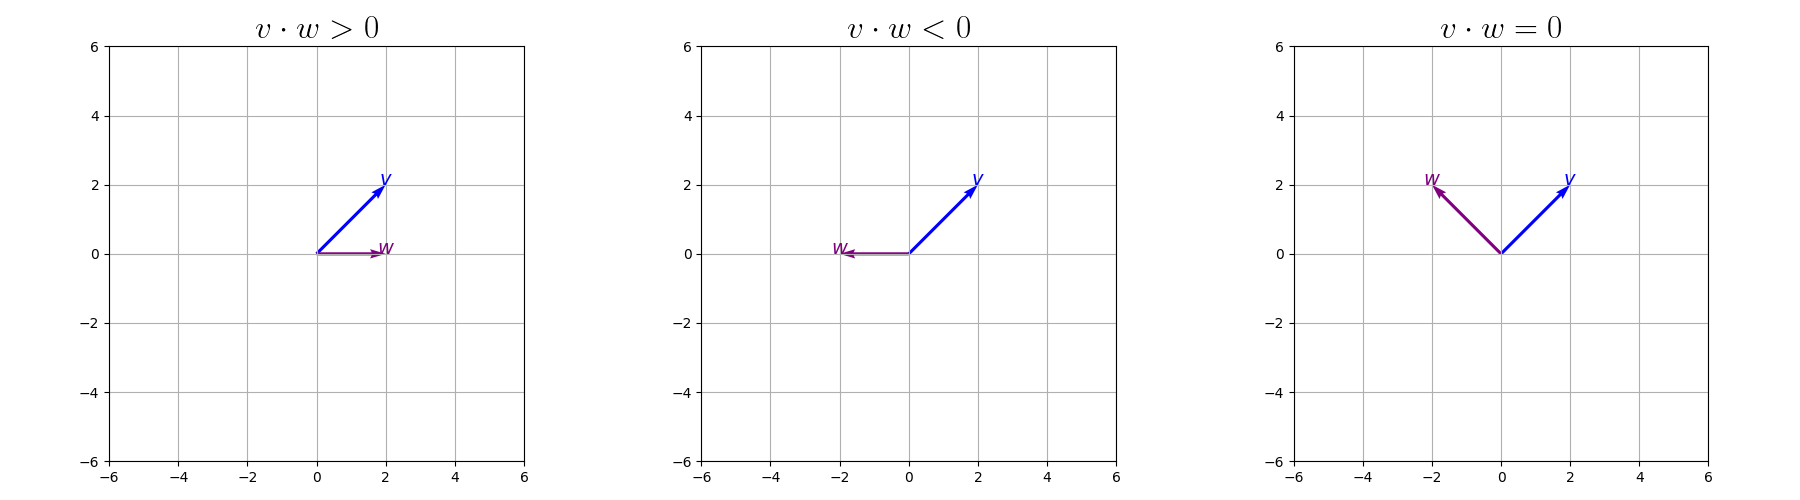
\includegraphics[width=140mm,scale=0.5]{images/transformers_images/dot_product_demo.png}
            
            
            \caption*{We can see here what we mean by "similar" or "dissimilar".}
        \end{figure}

        \begin{clarification}
            You can use $S_C(u,v)$ to measure the \gren{similarity} between two vectors, ignoring magnitude.

            But for simplicity, we'll skip the \purp{normalizing} step, and just take the \vocab{dot product}:

            \begin{equation*}
                S_D(u,v) = u \cdot v = u^\top v
            \end{equation*}
        \end{clarification}

        

        We're getting closer to a computable form:

        \begin{equation}
            \overbrace{ 
                (v_a \cdot v_b) \text{ is \orgg{large}}
            }^{\text{ \lblu{Similar vectors}}}
            \;\;\iff\;\; 
            \text{$a$ and $b$ are \gren{semantically similar words}}
        \end{equation}



    \phantom{}

    \subsection{Semantic Similarity and Word Frequency}

        The "right side" of our expression is a bit trickier: how do you compute which words have \gren{similar meanings}?

        We can't directly turn "meaning" into a number. But instead, we'll focus on a different concept, that might help us predict similarity:

        \begin{itemize}
            \item \miniex Earlier, we showed that "sweet and "sugar" were related, by referencing the fact that "\orgg{sugar tastes sweet}".

            \item While our machine might not understand the concept, it can see that "sugar" and "sweet" showed up \gren{together} in a sentence.
                \note{How much do/can large language models "understand" what they're saying? Lots of very smart people continue to argue exactly how much they know.}
        \end{itemize}

        Often, words that are related, show up in the same sentences, or paragraphs. So, we'll try to use this to our advantage:

        \begin{equation*}
            \text{$a$ and $b$ are \gren{semantically similar words}}
            \;\;\xLeftrightarrow{\text{maybe?}}\;\; 
            \text{$a$ and $b$ \purp{frequently} show up together}
        \end{equation*}

        These two aren't \textit{actually} equivalent, but we hope that we can use one to predict the other.\\

        \begin{concept}
            We can predict which words might be \orgg{more similar} by observing \purp{how often} they show up \gren{together} in a body ("corpora") of text.

            \begin{itemize}
                \item When two words occur \orgg{together} in a context, we call this \gren{co-occurrence}.
                \item Thus, we're measuring \vocab{frequency of co-occurrence}.
            \end{itemize}

            If two words show up near each other more frequently, we predict that they might be \gren{more similar}.

        \end{concept}

        This kind of word embedding is often called "\vocab{word2vec}", named after a particular set of algorithms that use this approach.
            \note{Sometimes, "word2vec" is used to reference any technology that creates word embeddings. But this isn't always technically accurate.}

        \begin{itemize}
            \item \miniex The words "quantum" and "physics" go together often. So do the words "rain" and "weather".\\
        \end{itemize}

        \begin{clarification}
            We \purp{don't actually know} for certain that, if two words often show up together, they have \orgg{related meanings}.

            But, in practice, we find that "\vocab{frequency of co-occurrence}" is a \gren{surprisingly good} measure of similarity.
        \end{clarification}

        Because we're talking about frequency, we'll consider the \gren{probability} of seeing both words together.

        \begin{equation*}
            \text{$a$ and $b$ are \gren{semantically similar words}}
            \;\;\xLeftrightarrow{\text{maybe?}}\;\; 
            \text{P \big( $a$ and $b$ \purp{occur together} \big) is \orgg{high}}
        \end{equation*}

        Finally, we have something closer to math:

        \begin{equation*}
            \overbrace{
                v_a \cdot v_b \text{ is \orgg{large}}}
            ^{\text{Similar vectors}}
            \;\;\iff\;\; 
            \overbrace{
                \text{P \big( $a$ and $b$ \purp{occur together} \big) is \orgg{high}}}
            ^{\text{Similar words}}
        \end{equation*}

        Now, we have some "mathematical" concepts: we can start using these to create mathematical \textbf{objects}.


    \phantom{}
    
    \subsection{Clarifying our probability}

        In order to proceed, we need to be a little more specific.

        \begin{equation*}
            \overbrace{
                (v_a \cdot v_b) \text{ is \orgg{large}}}
            ^{\text{Similar vectors}}
            \;\;\iff\;\; 
            \overbrace{
                \text{P \big( $a$ and $b$ \purp{occur together} \big) is \orgg{high}}}
            ^{\text{Similar words}}
        \end{equation*}

        
        The dot product is already an equation, so the left side is fine.

        \phantom{}
        
        The right side is all we need to clear up: "P \big( $a$ and $b$ \purp{occur together} \big)" is a bit \gren{vague}. 
            \note{One interpretation would be: "if we look at a random phrase, how often do we have words $a$ and $b$?"

            \phantom{}
            
            But we only care whether $a$ and $b$ are together/separate: we don't care about sentences containing neither.}
        
        \begin{itemize}
            \item We want to know if $a$ and $b$ tend to show up \orgg{together}, rather than \purp{separately}.
        \end{itemize}

        Here's a concrete way to say this: "\gren{if} we find one word, \purp{how often} do we find the other nearby?"\\

        \begin{concept}
            To predict how \gren{similar} words $a$ and $b$ are, we want to compute how often they \vocab{co-occur}.

            \begin{itemize}
                \item One way to phrase this: "\gren{given} that we find $a$, what are the \purp{chances} we find $b$ nearby?"
            \end{itemize}

            \begin{equation*}
                \given{b \text{ nearby} }{a \text{ found}}
            \end{equation*}
        
        \end{concept}

        \begin{equation*}
            \overbrace{ 
                (v_a \cdot v_b) \text{ is \orgg{large}}
            }^{\text{ \lblu{Similar vectors}}}
            \;\;\iff\;\; 
            \overbrace{
                \text{ $\given{b \text{ nearby} }{a \text{ found}}$  is \orgg{large}}}
            ^{\text{\lblu{Occur together frequently}}}
        \end{equation*}

        We're getting warmer! 
        
        \begin{itemize}
            \item We "\purp{find}" $a$ at index $t$: 
                \note{$w_t$ is the $\nth{t}$ word in our passage.}

                \begin{equation}
                    w_t=a
                \end{equation}

            \item Now, let's define what it means for $b$ to be "\gren{nearby}".\\
        \end{itemize}


        \begin{definition}
            In a text, we may want to find the "context" for \gren{center word} $w_t$: we want all of the words \orgg{nearby}.

            \begin{itemize}
                \item We'll use the $c$ nearest words on either side: these are our \purp{context words}. $c$ is our \vocab{maximum skip distance}.
            \end{itemize}

            This collection of $2c+1$ words is called our \vocab{context window}.

            \begin{equation*}
                \begin{matrix}
                    \cdots & w_{t-4} & 
                    \overbrace{
                    \begin{matrix}
                        \pur{w_{t-3}} & \pur{w_{t-2}} & \pur{w_{t-1}} &
                        \grn{w_t} & 
                        \pur{w_{t+1}} & \pur{w_{t+2}} & \pur{w_{t+3}}
                    \end{matrix} 
                    }^{\text{  Context window for $c=3$}}
                    & w_{t+4} & \cdots
                \end{matrix}
            \end{equation*}
            
        \end{definition}

            \note{We call $c$ our "maximum skip distance", because it's the largest number of words we can "skip" over, starting from $w_t$. 
            
            \phantom{}
            
            We're allow to move over by $c$ words, in either direction.}

        \begin{itemize}
            \item Notice the similarity to the filter size from Convolution: we still have an idea of "locality".
        \end{itemize}


        \phantom{}

        So, we want to look for $b$ in our context window. There are two ways we can turn this into a probability:

        \begin{itemize}
            \item You check all of the context words \orgg{at the same time}:

            \begin{equation}
                \begin{matrix}
                    \cdots & w_{t-3} & 
                    \overbrace{
                    \begin{matrix}
                        \pur{w_{t-2}} & \pur{w_{t-1}} & \grn{w_t} & \pur{w_{t+1}} & \pur{w_{t+2}}
                    \end{matrix} 
                    }^{\text{ All words within $c=2$ context window}}
                    & w_{t+3} & \cdots
                \end{matrix}
            \end{equation}

            \item You check \gren{one word at a time}: $j$ units to the right/left.

            \begin{equation}
                \begin{matrix}
                    \cdots & w_{t-3} & 
                    \overbrace{
                    \begin{matrix}
                        \blu{w_{t-2}} & w_{t-1} & \red{w_t} 
                    \end{matrix} 
                    }^{\text{Only $w_{t-2}$. Thus, $j=-2$}}
                    & w_{t+1} & w_{t+2}
                    & w_{t+3} & \cdots
                \end{matrix}
            \end{equation}
        \end{itemize}

        For now, it's easier to use the latter approach: \gren{each index} has a \purp{separate probability}.\\

        \begin{concept}

            We measure the \vocab{co-occurrence} of $a$ and $b$ by asking:

            \begin{itemize}
                \item "\orgg{Given} that we find $a$ at index $t$...

                \begin{equation*}
                    \grn{w_t=a}
                \end{equation*}
                
                \item what are the \orgg{chances} that we find $b$ at index $t+j$?"
                
                \begin{equation*}
                    \pur{w_{t+j} = b}
                \end{equation*}
            \end{itemize}

            With this, we find our result:

            \begin{equation*}
                \given{ \pur{w_{t+j} = b} }{ \grn{w_t=a} }
            \end{equation*}
            
        \end{concept}

        We did it! This is a clear, explicit probability.

        \begin{equation*}
            \overbrace{ 
                (v_a \cdot v_b) \text{ is \orgg{large}}
            }^{\text{ \lblu{Similar vectors}}}
            \;\;\iff\;\; 
            \overbrace{
                \given{ \pur{w_{t+j} = b} }{ \grn{w_t=a} } \text{ \quad is \orgg{large}}}
            ^{\text{\lblu{Occur together frequently}}}
        \end{equation*}

        \begin{notation}
            We can make this notation a little denser: 

            \begin{equation*}
                \given{ \pur{w_{t+j} = b} }{ \grn{w_t=a} }
                \quad=\quad
                \given{ b }{ a }_j
            \end{equation*}

            This assumes that $t$ \redd{doesn't} affect our probability: it doesn't matter \gren{where} we found $a$, just \purp{how far away} $b$ is (and on which side).

            \begin{itemize}
                \item This is a reasonable assumption for our purposes.
            \end{itemize}
        \end{notation}




    \phantom{}

    \subsection{Computing predicted probabilities}

        How do we turn a \gren{real number} $v_a \cdot v_b$ into a \purp{probability} $P\big(b \; | \; a\big)_j$? 

        \begin{itemize}
            \item $P\big(b \; | \; a\big)_j$ is the chance of finding $b$ at index $t+j$, if $a$ is at index $t$.

            \begin{equation}
                \begin{matrix}
                    \cdots & w_{t-3} & 
                    \overbrace{
                    \begin{matrix}
                        \blu{w_{t-2}} & w_{t-1} & \red{w_t} 
                    \end{matrix} 
                    }^{\text{What word is at $w_{t-2}$? Is it $b$?}}
                    & w_{t+1} & w_{t+2}
                    & w_{t+3} & \cdots
                \end{matrix}
            \end{equation}
            \item So, we need to compare $b$ to every other word that we could find at $t+j$: this is a \orgg{multi-class problem}, using the \vocab{softmax function}.
                \note{We have one class for each possible word we could find at $t+j$.}
        \end{itemize}

        \begin{equation}
            \operatorname{Softmax}(z_k) = \frac{e^{z_k}}{ \sum_i e^{z_i}}
        \end{equation}

        Let's review the concept behind "softmax":\\

        \begin{concept}
            Suppose that we have \purp{$n$ possible words} ($n$ "classes"), and we want to figure out which one is \gren{correct}.
            
            The \vocab{$\nth{k}$ class} has a score, \org{$z_k$}, used to compute probability.

            \begin{itemize}
                \item The bigger $z_k$ is, the \purp{more likely} $k$ is to be the \gren{correct class}.
            \end{itemize}

            \phantom{}

            To keep it \gren{positive}, $z_k$ is converted to \org{$e^{z_k}$}: each $e^{z_i}$ competes to see which class is more likely.

            \begin{itemize}
                \item To create a probability, we \purp{compare} the score of class $k$ to all of our other classes, using \vocab{softmax}.
            \end{itemize}

            \begin{equation*}
                \overbrace{
                    e^{z_k}}^{\text{\lblu{Class k}}} 
                \text{\; vs \;} 
                \overbrace{ 
                    \sum_i e^{z_i} }^{\text{\lblu{All classes}}}
                \quad \quad \Longrightarrow \quad \quad  \operatorname{Softmax}(z_k) = \frac{e^{z_k}}{ \sum_i e^{z_i}}
            \end{equation*}
            
        \end{concept}

        \begin{itemize}
            \item We repeat this process for every possible word $i$, to get all of our predictions.
        \end{itemize}

        Now, the big question: what is $z_k$?

        \begin{equation*}
            \overbrace{ 
                (v_a \cdot v_b) \text{ is \orgg{large}}
            }^{\text{ \lblu{Similar vectors}}}
            \;\;\iff\;\; 
            \overbrace{
                \given{ \pur{w_{t+j} = b} }{ \grn{w_t=a} } \text{ \quad is \orgg{large}}}
            ^{\text{\lblu{Occur together frequently}}}
        \end{equation*}

        $z_k$ and $(v_a \cdot v_b)$ serve the \vocab{same purpose}:

        \begin{itemize}
            \item Large \gren{dot product} predicts high probability.
            \item Large \pur{$z_k$} predicts high probability.
        \end{itemize}

        So, we can use our dot product as a "score" $z_k$:

        \begin{equation}
            z_b = \red{v_a} \cdot \grn{v_b}
        \end{equation}

        Now, we can plug this into our probability equation!\\

        \begin{kequation}
            The \gren{more similar} (bigger dot product) $a$ and $b$ are, the \purp{more likely} we predict to find them together.

            \begin{itemize}
                \item We use a \vocab{softmax} to compute this probability for each possible word $b$.
            \end{itemize}

            \begin{equation*}
                    \given{ \grn{w_{t+j} = b} }{ \red{w_t=a} } 
                    \quad=\quad
                    \frac{e^{\red{v_a} \cdot \grn{v_b}} }{ \sum_i e^{\red{v_a} \cdot \blu{v_i} }}
            \end{equation*}

            Or, in alternate notation: 
            
            \begin{equation*}
                \given{ \grn{b} }{ \red{a} } 
                \quad=\quad
                \frac{  \phantom{ \Bigg|} 
                \exp \Big(\red{v_a} \cdot \grn{v_b}\Big) }
                {\phantom{ \Bigg|}
                \sum_{\blu{i}} \exp \Big(\red{v_a} \cdot \blu{v_i} \Big) }
            \end{equation*}
        \end{kequation}

        Ta-da! We've combined two separate concepts into a single equation.
            \note{Note that, in both top and bottom, we keep \red{$v_a$}: we're considering every possible word for \blu{$w_{t+j}$}, while we \textit{know} \red{$w_t=a$}.}



    \phantom{}

    \subsection{Skip-gram approach: Training our word2vec model}

        One remaining issue: this equation doesn't tell us what the "true" probabilities are: they tell us the probability that our model \purp{predicts}.
        
        \begin{itemize}
            \item Now, we have to choose a \gren{good model} (word embedding).\\
        \end{itemize}
        
        \begin{clarification}
            Our equation is $\given{ \grn{w_{t+j} = b} }{ \red{w_t=a} }$ is our \orgg{estimation} for the probability.

            \begin{itemize}
                \item The real probabilities could be \purp{different}: we'll design our word embedding to give us the most \gren{accurate probabilities}.
            \end{itemize}
        \end{clarification}

        First: what does our model look like? How do we even \orgg{generate} word embeddings?

        \begin{itemize}
            \item Often, we rely on a neural network.\\
        \end{itemize}

        \begin{definition}
           We have two common \vocab{models for word embedding} ($\theta$):

            \begin{itemize}
                \item Separately assigning a \gren{vector} to each word.
                \item Using a shared \purp{neural network} to embed every word as a vector.
            \end{itemize}

            Our neural network uses \gren{parameters} $\theta$. We'll use $\theta$ to represent our embedding, that we want to \orgg{train}.

            \begin{equation*}
                \grn{w} \xlongrightarrow{\theta} v_{\grn{w}}
            \end{equation*}
        \end{definition}

        How do we pick a good model? 

        \begin{itemize}
            \item We'll \gren{train} our embedding $\theta$, so that our \purp{probabilities} are as accurate as possible.
        \end{itemize}

        As we established, our problem is multi-class classification:\\

        \begin{concept}
            \textit{Review from Classification chapter}

            For \vocab{multi-class classification}, we use the \gren{negative log-likelihood multiclass} (NLLM) equation to compute \purp{loss}:

            \begin{equation*}
                \loss_{NLLM}
                (\red{g} , \blu{y})
                =
                -\sum_{i=1}^n
                y_i \log(g_i)
            \end{equation*}

            $y$ is a one-hot vector, so all terms of the sum except the "correct" term $i=k$ cancel out to 0:

            \begin{equation*}
                -\blu{y_k} \log(\red{g_k})
                \qquad \xlongrightarrow{y_k=1  } \qquad
                -\log(\red{g_k})
            \end{equation*}
        \end{concept}

        $g_k$ is the probability we assigned to the correct answer.

        Next, we need training data: a body of \purp{text}.

        \begin{itemize}
            \item For an example, let's visit index $t$ in the text: this is the center of our \vocab{context window}. 
            \item $a$ is replaced by whatever word we find at that index: \red{$w_t$}. We still want to predict \blu{$w_{t+j}$}.
        \end{itemize}

        \begin{equation}
            \begin{matrix}
                \cdots & w_{t-3} & 
                \begin{matrix}
                    w_{t-2} & w_{t-1} & \red{w_t} 
                \end{matrix} 
                & \cdots & \blu{w_{t+j}}
                & w_{t+j+1} & \cdots
            \end{matrix}
        \end{equation}

        How good is our word embedding? According to NLLM: "how likely were we to correctly predict $w_{t+j}$?"

        \begin{equation*}
            \loss_{NLLM}(\red{g},\blu{y}) = -\log \Big(
                \given{\text{\grn{Correct word for index $t+j$}}}{\red{w_t}} 
            \Big) 
        \end{equation*}

        The correct word for index $t+j$ would be... $w_{t+j}$. We can read the outcome from the text, and use our model to check how \purp{likely} we thought that outcome was.

        \begin{equation*}
            \loss_{NLLM}(\red{g},\blu{y}) = -\log \Big(
                \overbrace{
                \given{\grn{w_{t+j}}}{\red{w_t}} 
                }^{\text{How likely we thought $w_{t+j}$ was, based on model}}
            \Big) 
        \end{equation*}

        Note that, the higher this probability is (the more sure we are of the correct answer), the closer the loss gets to 0.\\

        \begin{kequation}
            We train our \vocab{word embedding} $\theta$ by \purp{maximizing} the probability $\mathbf{P}(\grn{w_{t+j}} \quad|\quad \red{w_t})$ of predicting the \gren{correct word} in each spot.

            In our case, we want to \purp{minimize}

            \begin{equation*}
                \loss_{NLLM}(\theta,j) = -\log \Big(
                    \given{\grn{w_{t+j}}}{\red{w_t}} 
                \Big) 
            \end{equation*}
            where

            \begin{equation*}
                \given{ \grn{b} }{ \red{a} } 
                \quad=\quad
                \frac{  \phantom{ \Bigg|} 
                \exp \Big(\red{v_a} \cdot \grn{v_b}\Big) }
                {\phantom{ \Bigg|}
                \sum_{\blu{i}} \exp \Big(\red{v_a} \cdot \blu{v_i} \Big) }
            \end{equation*}
        \end{kequation}

        Now, we know how to compute these odds for a \purp{single index}, $t+j$. We want to repeat this process for the rest of our context window:


        \begin{equation}
            \begin{matrix}
                \cdots & w_{t-3} & 
                \overbrace{
                \begin{matrix}
                    \pur{w_{t-2}} & \pur{w_{t-1}} & \grn{w_t} & \pur{w_{t+1}} & \pur{w_{t+2}}
                \end{matrix} 
                }^{\text{ All words within $c=2$ context window}}
                & w_{t+3} & \cdots
            \end{matrix}
        \end{equation}

        \begin{kequation}
            We can find the \purp{total loss} of our embedding $\theta$, over our entire \vocab{context window}, by adding up the loss from each \gren{context word}.
            
            This includes all of the indices $(t+j)$, going from $j=-c$ to $j=+c$. Meaning, we want 

            \begin{itemize}
                \item \org{$|j| \leq c$} (within window) 
                \item \pur{$j \neq 0$} (don't want to compare $w_t$ with itself)
            \end{itemize}

            

            \begin{equation*}
                \loss_{t}(\theta) = - \sum_{\org{|j| \leq c}}^{\pur{j \neq 0}}
                \log \Big(
                    \given{\grn{w_{t+j}}}{\red{w_t}} 
                \Big) 
            \end{equation*}
        \end{kequation}

        One more modification: the loss function above only computes loss for a \gren{single context window}.

        But, for a passage of text, there are many possible context windows: all we have to do is shift our target word, $w_t$.

        \begin{itemize}
            \item \miniex Below, with $c=2$, we'll show all of our possible context windows: 
                \note{Target word is red, context words are blue.}
        \end{itemize}

        \begin{equation}
            \begin{matrix}
                \text{\red{This} \blu{is a} sample sentence} \\
                \text{\blu{This} \red{is} \blu{a sample} sentence} \\
                \text{\blu{This is} \red{a} \blu{sample sentence}} \\
                \text{This \blu{is a} \red{sample} \blu{sentence}} \\
                \text{This is \blu{a sample} \red{sentence}} 
            \end{matrix}
        \end{equation}

        We'll average the loss over \orgg{all context windows}.
            \note{We'll ignore negative indices, so we don't cause problems when $t=0$ or $t=T$.}\\

        \begin{kequation}
            Take a body of text with $T$ words, and a \purp{context window} with a \gren{max skip distance} of $c$. We use word embedding $\theta$.

            Our \orgg{objective function} $J(\theta)$ for the \vocab{skip-gram word2vec} algorithm, over the entire passage, is:

            \begin{equation*}
                J(\theta) = \frac{1}{T} \sum_{t=1}^T \loss_{t}(\theta)
            \end{equation*}

            or,

            \begin{equation*}
                J(\theta) = -\frac{1}{T} \sum_{t=1}^T 
                \quad
                \Bigg( \quad
                    \sum_{\org{|j| \leq c}}^{\pur{j \neq 0}}
                    \log \Big(
                        \given{\grn{w_{t+j}}}{\red{w_t}} 
                    \Big) \quad
                \Bigg)
            \end{equation*}
        \end{kequation}

            

        This is the completed loss function that we can use to train our embedding.\\

        \begin{concept}
            We can train our \gren{embedding} $\theta$ using our \purp{loss function} $J$, via \vocab{gradient descent}.

            \begin{equation*}
                \grn{\theta'} = \grn{\theta} - \eta \nabla_{\grn{\theta}}\pur{J}
            \end{equation*}

            \begin{itemize}
                \item If we're using a \orgg{neural network} to create embeddings, we'll need \phantom{fillertonextline} \vocab{back-propagation} to train.
            \end{itemize}
        \end{concept}




    \pagebreak




    \subsection{Issues with skip-gram}

        There are a few problems worth addressing. First, look again at our equation:

        \begin{equation*}
                \given{ \grn{w_{t+j} = b} }{ \red{w_t=a} } 
                \quad=\quad
                \frac{e^{\red{v_a} \cdot \grn{v_b}} }{ \sum_i e^{\red{v_a} \cdot \blu{v_i} }}
        \end{equation*}

        Something might strike you: our probability is \purp{totally independent} of which index $t+j$ we want to predict.

        \begin{itemize}
            \item That means, our model would make the exact same prediction for every nearby word.
            \item This is more easily resolved in our transformer model, so we won't worry about it for now.\\
        \end{itemize}

        \begin{concept}
            Our \purp{probability} calculation in skip-gram is \gren{independent} of the \vocab{skip distance} $j$ between words $w_t$ and $w_{t+j}$.

            \begin{itemize}
                \item All words within the \vocab{context window} have the \orgg{same probability distribution}.
            \end{itemize}
        \end{concept}


        Another problem: if "more \gren{similar}" means "more likely to \orgg{co-occur}", doesn't that suggest that we would expect a word to appear with itself, really often?

        \begin{itemize}
            \item This would be true for every word: nothing can be more similar to a vector than itself, after all.

            \item Our solution is to just \purp{exclude} $w_t$ from predictions about nearby words.\\
        \end{itemize}

        \begin{concept}
            The most similar word to $w_t$, is \orgg{itself}!

            \begin{itemize}
                \item So, we often \purp{exclude} $w_t$ from predictions.
            \end{itemize}
        \end{concept}


        Another problem: our objective function $J(\theta)$ includes a logarithm. To optimize $\theta$, we'd need to compute its \purp{derivative}.

        \begin{itemize}
            \item This becomes really expensive, especially when our vocabulary can have millions of words.

            \item Our solution is to "\orgg{prune}"/remove a lot of words from our probability calculation.
                \note{We can predict in advance, that some words don't need to be included.}\\
        \end{itemize}
            
        \begin{concept}
            \vocab{Skip-gram} can become expensive to train, when the \gren{vocabulary} becomes too large.

            \begin{itemize}
                \item So, we \orgg{prune} some unlikely words in our vocabulary, to speed up our \purp{predictions}.
            \end{itemize}
        \end{concept}


    \subsection{Tokenization}

        One more concern: so far, we've talked about predicting whole words, because it's easy to work with.

        \begin{itemize}
            \item But often, for language analysis, we break up words into parts, called \vocab{tokens}.

            \item These are the objects we study/predict, rather than whole words.\\
        \end{itemize}

        \begin{definition}
            Rather than using/predicting entire \orgg{words}, we use \purp{small parts of words}, called \vocab{tokens}.

            \begin{itemize}
                \item A "token" is the \gren{smallest unit} in our language model.
            \end{itemize}
        \end{definition}

        \begin{itemize}
            \item \miniex You might break up the word "eating" into "eat" and "ing": both are meaningful, by themselves.
                \note{This is another reason our vocabulary becomes so big: we're not just considering every word, we're including smaller pieces of words.}

            \item This process of turning words into tokens is called \vocab{tokenization}.
        \end{itemize}

        While "tokens" are used more often than "words", words often make for better examples, so we'll keep using them through the rest of this chapter.\\

        \begin{clarification}
            We'll continue using words (instead of tokens) for examples, when it's convenient.
        \end{clarification}

         





    

    \pagebreak
    
    \subsection{"Adding" words together}

        Our word2vec system works under the hope that these vector embeddings can accurately represent the \purp{meanings} of words.

        \begin{itemize}
            \item In practice, this assumption works \gren{surprisingly well}, for being so simple.
        \end{itemize}

        One example is the idea of "\orgg{adding}" words together. Normally, it's hard to say how to "add words" together, but we \textit{do} know how to add \purp{vectors}.

        Consider the following example:

        \begin{equation}
            v_{king} - v_{man} + v_{woman}  \quad\approx\quad v_{queen}
        \end{equation}

        This sort of reasoning makes sense to most english speakers: 

        \begin{equation}
            \overbrace{ v_{king} - v_{man} }^{\text{ruler}} \;\;+\;\; v_{woman} 
            \quad\approx\quad \overbrace{v_{queen}}^{\text{female ruler}}
        \end{equation}

        We can repeat this process for other words:
            \note{Paris is the capital of France, and Rome is the capital of Italy.}

        \begin{equation}
            v_{paris} - v_{france} + v_{italy}  \quad\approx\quad v_{rome}
        \end{equation}

        \begin{concept}
            Transforming a word into a \orgg{vector} allows you to use vector operations, like \gren{addition} and \purp{subtraction}.

            \begin{itemize}
                \item The result can be surprisingly \gren{meaningful}, for some word combinations.
            \end{itemize}

            This approach doesn't always work, but the fact that it works \textit{sometimes} suggests that our vectors might capture real information about the "\purp{meanings}" of words.
        \end{concept}

        That said, this approach is often an over-simplification:\\

        \begin{concept}
            Reducing a word to a \purp{single vector} can cause problems, because the same word might change its meaning, based on \gren{context}.
        \end{concept}

        \begin{itemize}
            \item \miniex For example, the word "bank" has a very different meaning when you compare "bank account" to "river bank".
        \end{itemize}

        This idea of "context" is what we hope to solve next.

    

\pagebreak
    
\section{Attention}

    Our \orgg{word embedding} technique has given us a basic way to talk about which words are "\gren{related}".

    \begin{itemize}
        \item We can even use this to learn some about the "\purp{meanings}" of words.
    \end{itemize}

    But there's some work to be done:\\

    \begin{concept}
        Our \vocab{word embedding} technique has two major problems, for representing the \purp{meanings} of words:

        \begin{itemize}
            \item There's a lot of information we're \purp{missing}: \gren{similarity} to other words isn't enough. We'll need a vector to represent that information.
    
            \item The meaning of a word is \orgg{contextual}: the sentence you put a word in, will affect its meaning.
        \end{itemize}
    \end{concept}

    

    It may not look like it, but our \purp{word embedding} technique has already given us the basic tools we need to solve these problems.

    Here's the basic idea, for how we handle each problem:\\

    \begin{concept}
        We'll create a system that solves both of these problems, using \purp{3 word embeddings}: \org{$v$}, \org{$k$}, and \org{$q$}.

        \phantom{}

        \begin{itemize}
            \item We'll \orgg{embed} \gren{information} about each word in a \vocab{value vector} $v$.
    
            \item When finding the \purp{meaning} of a word, we'll calculate \gren{context} from nearby words.
    
            \begin{itemize}
                \item We'll use \gren{word similarity} to figure out which parts of the context are \purp{most important}.
                
                \item For this purpose, word will need \orgg{two embeddings}: a \vocab{key vector} $k$, and a \vocab{query vector} $q$.
            \end{itemize}
        \end{itemize}

        \phantom{}

        The result is a powerful model called the \vocab{attention mechanism}.
    \end{concept}

    This description is over-simplified, which is why we'll need to go into detail below.

    

    




    \phantom{}

    \subsection{The Attention Mechanism: queries, keys}

        Let's consider an \purp{example}, to get used to the idea of $k$, $v$, and $q$.

        Suppose we want a general idea of what "mexican" food is like. We'll need to consider lots of foods, and take an \gren{average} of those we consider to be "mexican".
            \note{Admittedly, we're turning "mexican-ness" into a number, which can be a bit strange. 
            
            \phantom{}
            
            It may help to think this way: "if someone is talking about mexican food, how often are they talking about this food?"}

        \phantom{}

        This problem comes in three parts: let's consider the first two, "query" and "key".

        \begin{itemize}
            \item \vocab{Query $q$}: we're searching for "mexican" food. The word "mexican" is represented by a \purp{query vector} $q$. 
            
            \begin{itemize}
                \item This is like our previous \orgg{word2vec} embedding: if two vectors are similar, then we expect them to have similar/related \orgg{meanings}.
                \item So, we'll \gren{compare} $q$ to each food, to see which foods are 'close' to mexican.\\
            \end{itemize}

            \begin{definition}
                The \vocab{query vector} $q$ represents a word, that we're \gren{comparing} to \purp{several other words} ("keys").

                \begin{itemize}
                    \item It answers the question, "what kinds of words are we \orgg{searching} for?" 
                \end{itemize}

                Using word embeddings, we design $q$ to be "meaningful": similar words, should have similar vectors.
                
                \begin{itemize}
                    \item And we expect \purp{similar words} to be \gren{more relevant} to our query.
                \end{itemize} 
            \end{definition}

            \phantom{}

            \item \vocab{Key $k$}: Each food (apple, burrito, sushi...) has a \purp{key vector} $k$, representing it. 
            
            \begin{itemize}
                \item A \orgg{word2vec}-style embedding, just like the \orgg{query}.

                \item Combining $k$ and $q$ will tell us which foods are \gren{'more' mexican}.\\

            \end{itemize}

            \begin{definition}
                The \vocab{key vector} $k$ represents a word, that we want to \gren{compare} to \purp{the query} $q$.

                \begin{itemize}
                    \item It answers the question, "what kinds of searches does this word \orgg{match}"?
                \end{itemize}

                Because it's a word embedding, which encodes meaning, we expect that, if \purp{$k$ and $q$ are similar}, then our key word is \gren{more relevant} to our query.
            \end{definition}
        \end{itemize}

        Each embedding has a role: a \purp{query} is used to search for relevant words, and a \gren{key} is responding to that search, on behalf of one word.
            \note{Reminder that when we say "word", we're simplifying: we could talk about any kind of token.}

        \begin{concept}
            Another way we could view keys vs. queries:

            \begin{itemize}
                \item \orgg{Query vector $q$}: asks, "how relevant are these words/tokens \purp{to me}?"

                \item \orgg{Key vector $k$}: asks, "how relevant is my word \gren{to the query}?"
            \end{itemize}
        \end{concept}


        \phantom{}

        Notice that we've made a perspective shift, in how we view word embeddings:\\

        \begin{concept}
            When we were developing word2vec, we wanted \purp{similar vectors} to represent \gren{semantically similar} words.

            \begin{itemize}
                \item But, in this case, we're less focused on "similarity", than \orgg{relevance}.
            \end{itemize}

            We look for \purp{keys} that are the \orgg{most relevant} to our \gren{query}.

        \end{concept}

        These two ideas don't necessarily conflict, but they have somewhat different goals.

    \phantom{}

    \subsection{The parts of Attention: attention weights}

        How do we compute how similar $k$ and $q$ are? The same way as we did for word2vec: we use a \gren{dot product}.\\

        \begin{kequation}
            We can get a score for how \gren{relevant} the word $b$ is to word $a$, by taking the \purp{dot product} between \orgg{$b$'s key}, and \orgg{$a$'s query}.

            \begin{equation*}
                k_b \cdot q_a  
            \end{equation*}

            We can also write this as matrix multiplication:

            \begin{equation*}
                k \cdot q = k^Tq
            \end{equation*}
        \end{kequation}

        This gives us a "\orgg{score}": the higher $k \cdot q$ is, the more similar they are.

        \begin{figure}[H]
            \centering
            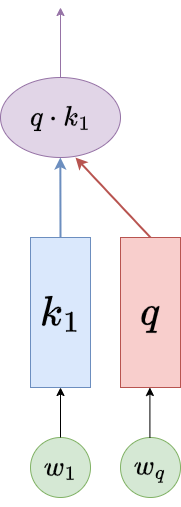
\includegraphics[width=0.1\linewidth]{images/transformers_images/k_dot_q.png}
            \caption*{We convert $w_1$ and $w_q$ into a key and query, respectively, before taking the dot product.}
        \end{figure}

        But we're not just considering one key word: we're considering \gren{all of of them}.

        \begin{itemize}
            \item In our "mexican food" example, we need to check every food, to see which ones best fit the category.
        \end{itemize}

        \begin{figure}[H]
            \centering
            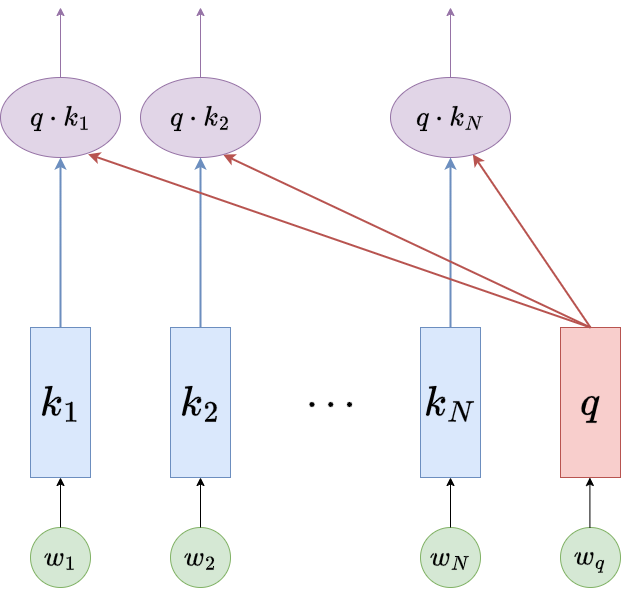
\includegraphics[width=0.3\linewidth]{images/transformers_images/k_dot_q_all.png}
            \caption*{We re-use our query $q$ for every single dot product.}
        \end{figure}

        How do we compare each of these keys?

        \begin{itemize}
            \item Once again, we'll reuse a tool from word2vec: \vocab{softmax}.\\
        \end{itemize}
        

        \begin{kequation}
            We can compute the relative \orgg{relevance} of a key $k_n$, by:

            \begin{itemize}
                \item \gren{Comparing} each key $k_i$ to $q$ ($k_i \cdot q$)

                \item Use \purp{softmax} to compute $p(k_n|q)$: given query $q$, how important is $k_n$?
            \end{itemize}


            \begin{equation*}
                    \given{ \grn{k_n} }{ \red{q} } 
                    \quad=\quad
                    \frac{ \phantom{\Big|}  e^{\grn{k_n} \cdot \red{q}} \phantom{\Big|}}
                    {\phantom{\Big|} \sum_i e^{\pur{k_i} \cdot \red{q} } \phantom{\Big|}}
            \end{equation*}

            $\given{ \grn{k_n} }{ \red{q} }$ tells you, "how much \orgg{attention} should $q$ pay to $k_b$"? 

            \begin{itemize}
                \item Thus, we call $\given{ \grn{k_n} }{ \red{q} }$ an \vocab{attention weight}.
            \end{itemize}
        \end{kequation}

        \begin{figure}[H]
            \centering
            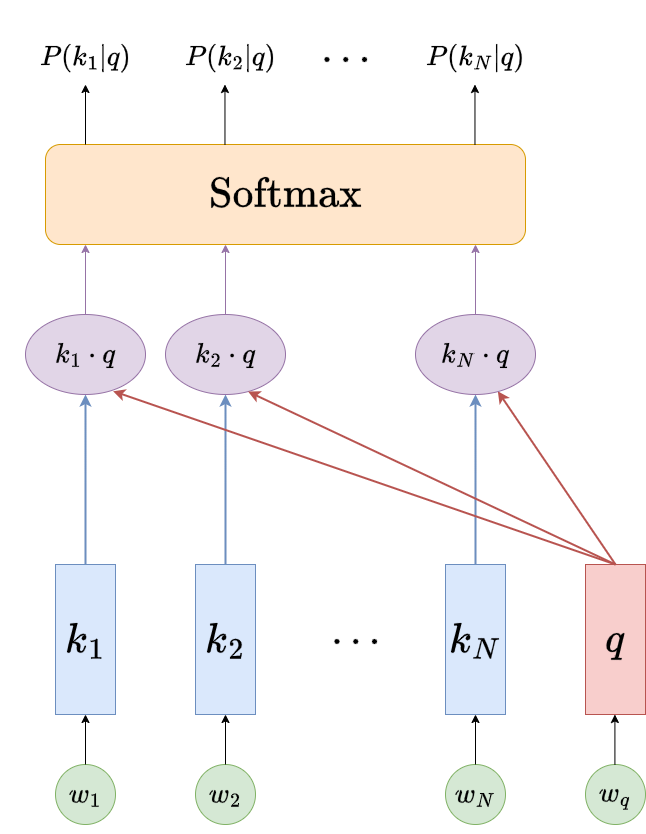
\includegraphics[width=0.3\linewidth]{images/transformers_images/softmax_attention.png}
            \caption*{Finally, we've converted each word into their "probability" of being relevant.}
        \end{figure}

        One notational thing: we can write this a bit more densely.

        \begin{itemize}
            \item So far, we've been computing $k^Tq$ for each $k_i$ term \gren{separately}.

            \item But, one benefit of matrix multiplication, is that we can \purp{combine multiple operations} into one.
        \end{itemize}

        First, we'll \gren{combine} all of our key vectors into a matrix $K$:

        \begin{equation}
            K = 
            \begin{bmatrix}
                \vertbar & \vertbar  & \     & \vertbar \\
                k_1 & k_2 & \ldots & k_N \\
                \vertbar & \vertbar  &        & \vertbar
            \end{bmatrix}
        \end{equation}

        With that, we can compute all of our dot products \purp{at the same time}:

        \begin{equation}
            K^Tq = 
            \begin{bmatrix}
                k_1 \cdot q \\ k_2 \cdot q \\ \vdots \\ k_N \cdot q \\
            \end{bmatrix}
        \end{equation}

        And we can combine all of these together into a softmax.\\

        \begin{kequation}
            By combining all of our keys into a matrix $K$, we can compute all of our \vocab{attention weights} \gren{at the same time}.

            \begin{equation*}
                \given{ \grn{K} }{ \red{q} }  \quad=\quad
                \begin{bmatrix}
                    \phantom{\Big|} 
                    \mathbf{P} \big( \grn{k_1} \;\big|\; \red{q} \big) \phantom{\Big|} \\
                    \phantom{\Big|}
                    \mathbf{P} \big( \grn{k_2} \;\big|\; \red{q} \big) 
                    \phantom{\Big|}\\
                    \vdots \\
                    \phantom{\Big|}
                    \mathbf{P} \big( \grn{k_N} \;\big|\; \red{q} \big) 
                    \phantom{\Big|}\\
                \end{bmatrix}
                \quad=\quad
                \operatorname{softmax} \big( \grn{K^T}\red{q} \big)
            \end{equation*}
        \end{kequation}


        \begin{figure}[H]
            \centering
            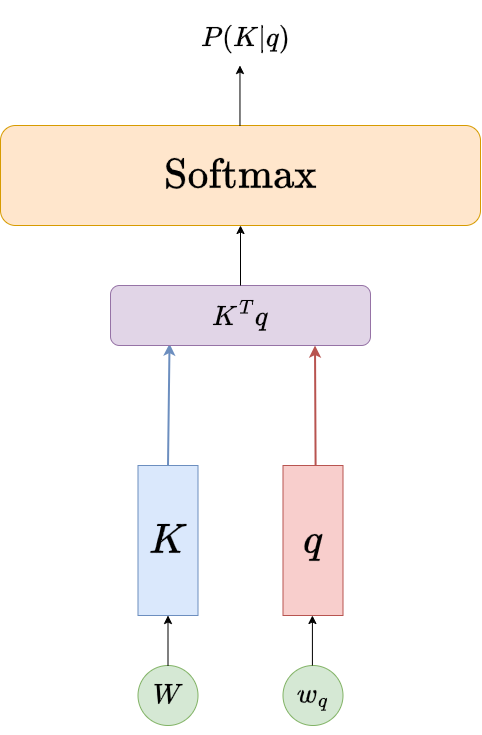
\includegraphics[width=0.3\linewidth]{images/transformers_images/condensed_attention_weights.png}
            \caption*{Now, our diagram is visually simpler, though it reflects the same information.}
        \end{figure}

        




    \phantom{}

    \subsection{The Attention Mechanism: values, attention}

        Now, we have a collection of \orgg{attention weights}: each one tells us relevant each word is to $q$.

        \begin{itemize}
            \item Now, we want to make them useful. Our original goal was to get an \gren{average} sense of what "mexican" food is like.
        \end{itemize}

        To make this concrete, we'll introduce our third embedding: the \purp{value vector}.

        \begin{itemize}
            \item \vocab{Value $v$}: Each food has a \purp{value vector}, directly storing information about a word.

            \begin{itemize}
                \item Unlike the key/query vectors, this embedding isn't based on \orgg{similarity} to other words.

                \item Instead, it usually contains more direct \purp{information} about our word: in this example, maybe it contains the price, calories, ingredients, etc.
                    \note{Note that, in a real model, value vectors are often "learned" during training. So, they won't always contain such simple, easily explained data.}\\
            \end{itemize}

            \begin{definition}
                The \vocab{value vector} $v$ represents a word, and stores useful \gren{information} that it can contribute to the \purp{query}.

                \begin{itemize}
                    \item It answers the question, "what useful data could this word contribute to the query?"
                \end{itemize}

                By \gren{adding together} the value vectors from each word \orgg{relevant} to the query, we can get an overall "\purp{averaged value}" for $q$.
            \end{definition}
        \end{itemize}

        \begin{figure}[H]
            \centering
            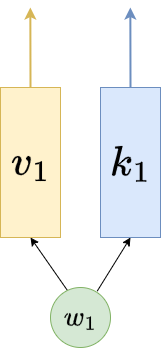
\includegraphics[width=0.1\linewidth]{images/transformers_images/value_key.png}
            \caption*{Each word has both a value and a key attached to it.}
        \end{figure}

        For our example, let's suppose that the value vector contains price, calories, and salt.

        \begin{equation}
            v_i = \begin{bmatrix}
                \text{price}_i \\ \text{cal}_i \\ \text{salt}_i
            \end{bmatrix}
        \end{equation}

        We want to get an "average" calorie count for mexican food.

        \begin{itemize}
            \item Some foods are \gren{common} for mexican food, and some are more rare.

            \item So, to get an average, we'll need to \orgg{emphasize} more "common" mexican food.
        \end{itemize}

        How do we do that? Using our \vocab{attention weights}: the larger the attention weight, the more "\orgg{relevant}" a food is to our mexican food calculation.

        If we use $q$ to represent \red{mexican} food, and $k_i$ is the \gren{key} for the $\nth{i}$ food, we get:

        \begin{equation}
            \text{cal}_{q} = 
            \overbrace{
                \sum_i P(\grn{k_i}|\red{q}) \;\; \text{cal}_{i}
            }^{\text{Weighted average}}
        \end{equation}

        Rather than repeating this process for each row of $v$, we can just do a \vocab{weighted average} of the whole vector, at the same time:

        \begin{equation}
            v_{q} = 
                \sum_i P(\grn{k_i}|\red{q}) \; v_{i}
        \end{equation}

        \begin{kequation}
            Each word $i$ has a \orgg{value vector} $v_i$, which represents all of the useful \gren{information} it can provide to the \purp{query}.

            \begin{itemize}
                \item We can use a \vocab{weighted average} to combine all of these value vectors together: this provides the "\purp{overall context}" for the query.

                \item Each value is weighted based on its \orgg{attention weight} $P(\grn{k_i}|\red{q}) $: how likely it is to be relevant.
            \end{itemize}

            \begin{equation*}
                v_{q} = 
                    \sum_i P(\grn{k_i}|\red{q}) \; v_{i}
            \end{equation*}

            This is the calculation for \vocab{attention}.
        \end{kequation}

        Just like we did for the $k_i \cdot q$ operation, we can re-write this in terms of matrix multiplication.

        \begin{itemize}
            \item We'll change from $P(\grn{k_i}|\red{q})$ to $P(\grn{K}|\red{q})$.
        

            \begin{equation*}
                \given{ \grn{K} }{ \red{q} }  \quad=\quad
                \begin{bmatrix}
                    \phantom{\Big|} 
                    \mathbf{P} \big( \grn{k_1} \;\big|\; \red{q} \big) \phantom{\Big|} \\
                    \phantom{\Big|}
                    \mathbf{P} \big( \grn{k_2} \;\big|\; \red{q} \big) 
                    \phantom{\Big|}\\
                    \vdots \\
                    \phantom{\Big|}
                    \mathbf{P} \big( \grn{k_N} \;\big|\; \red{q} \big) 
                    \phantom{\Big|}\\
                \end{bmatrix}
                \quad=\quad
                \operatorname{softmax}( \grn{K^T}\red{q})
            \end{equation*}

            \item We'll stack all of our value functions $v_i$ into a matrix $V$.

            \begin{equation}
                V = 
                \begin{bmatrix}
                    \vertbar & \vertbar  & \     & \vertbar \\
                    v_1 & v_2 & \ldots & v_N \\
                    \vertbar & \vertbar  &        & \vertbar
                \end{bmatrix}
            \end{equation}
        \end{itemize}

        Now, we can compute with every value vector at once:\\

        \begin{kequation}
            We can compute \vocab{attention} using matrix multiplication:

            \begin{equation*}
                \operatorname{Attention} \big( \red{q},\grn{K},\org{V} \big) 
                \quad=\quad 
                \org{V} \cdot \operatorname{softmax} \big( \grn{K^T}\red{q} \big)
            \end{equation*}

            Where $\operatorname{softmax} \big( \grn{K^T}\red{q} \big)$ computes our \purp{attention weights}.
        \end{kequation}

        \begin{figure}[H]
            \centering
            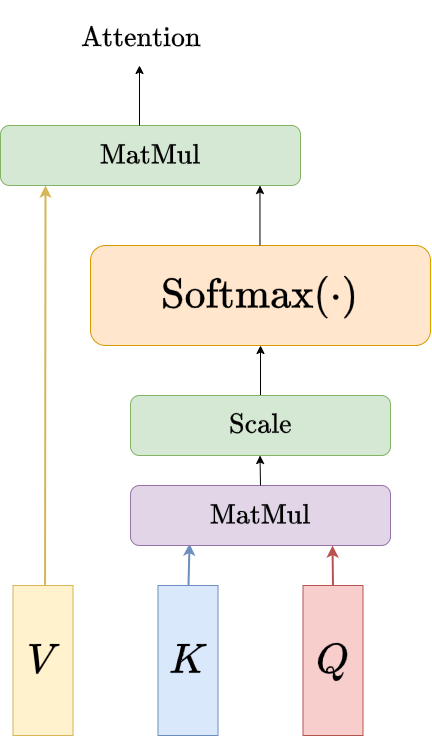
\includegraphics[width=0.3\linewidth]{images/transformers_images/condensed_attention.png}
            \caption*{We now have a completed representation of attention. The only thing missing: sometimes we normalize each dot product $k^T q$, before softmax.}
        \end{figure}

        With this, we can summarize the basic idea of attention:\\

        \begin{concept}
            \vocab{Attention} is a mechanism that allows you to \gren{combine} information from multiple tokens, weighting each token by how \purp{relevant} it is.

            This mechanism is broken into three parts:

            \begin{itemize}
                \item \orgg{Value vector $v$}: \gren{what information} are we trying to combine?

                \item \orgg{Query vector $q$}: what kinds of words are \purp{relevant} to this search?

                \item \orgg{Key vector $k$}: what kinds of searches is this word \gren{relevant} for?
            \end{itemize}

            Each token has a \purp{value vector} (information from that token), and a \gren{key vector} (used to compare this token to the query).
        \end{concept}

        Note that this isn't the \purp{only} way to do attention:\\

        \begin{clarification}
            There are multiple ways we can implement attention.

            \begin{itemize}
                \item For example, we use $k \cdot q$ to measure similarity, but we could \purp{replace} it with a different metric.
            \end{itemize}
        \end{clarification}

            \note{Reminder: a "metric" is just "a way of measuring something. The dot product is a \vocab{similarity metric} for vectors.}






    \pagebreak


    \subsection{Diagramming attention (\redd{Optional})}

        Above, we opted to use the "condensed" matrix notation, when introducing $V$ to the attention equation:

        \begin{figure}[H]
            \centering
            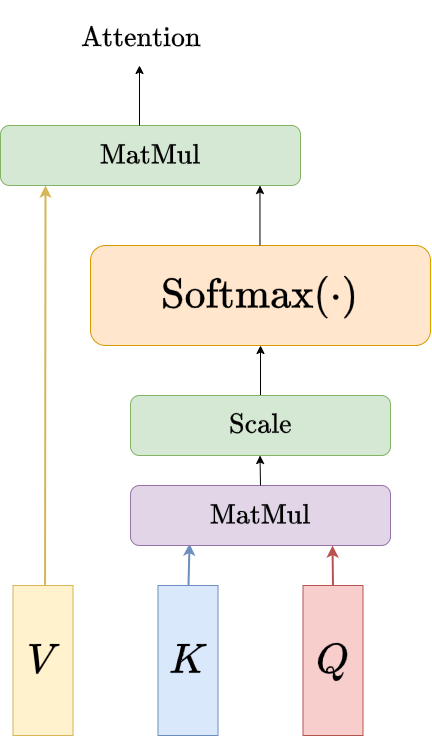
\includegraphics[width=0.2\linewidth]{images/transformers_images/condensed_attention.png}
            \caption*{We now have a completed representation of attention. The only thing missing: sometimes we normalize each dot product $k^T q$.}
        \end{figure}

        But sometimes, it's helpful to be able to see each individual key and value, $k_n$ and $v_n$. We'll create an alternate diagram following this format.

        \begin{figure}[H]
            \centering
            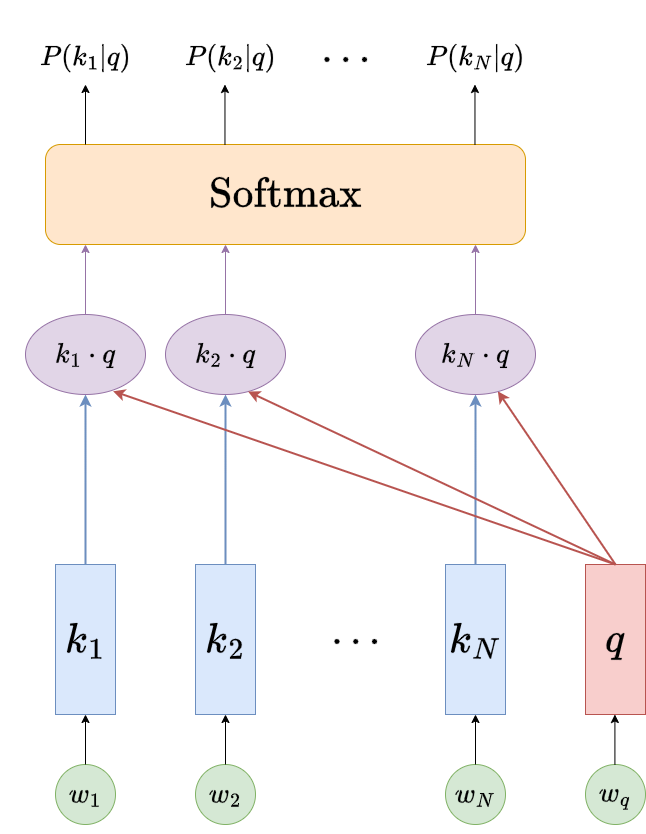
\includegraphics[width=0.3\linewidth]{images/transformers_images/softmax_attention.png}
            \caption*{We'll start from this diagram.}
        \end{figure}

        Each word $w_n$ not only has its own \gren{key}, but also its own \purp{value}.

        \begin{figure}[H]
            \centering
            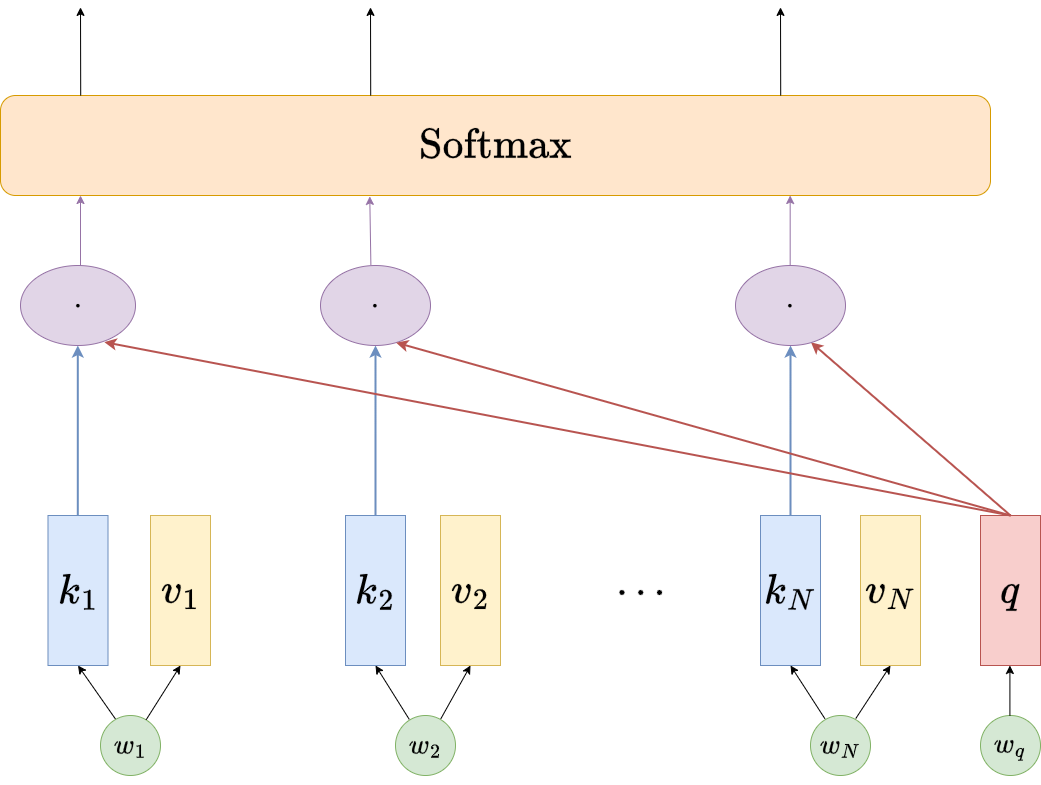
\includegraphics[width=0.45\linewidth]{images/transformers_images/softmax_value_vectors.png}
            \caption*{Each word produces a key and a value.}
        \end{figure}

        The notation here gets a bit... messy. We need to pair each weight $P(k_n|q)$ with its matching value, $v_n$.

        \begin{figure}[H]
            \centering
            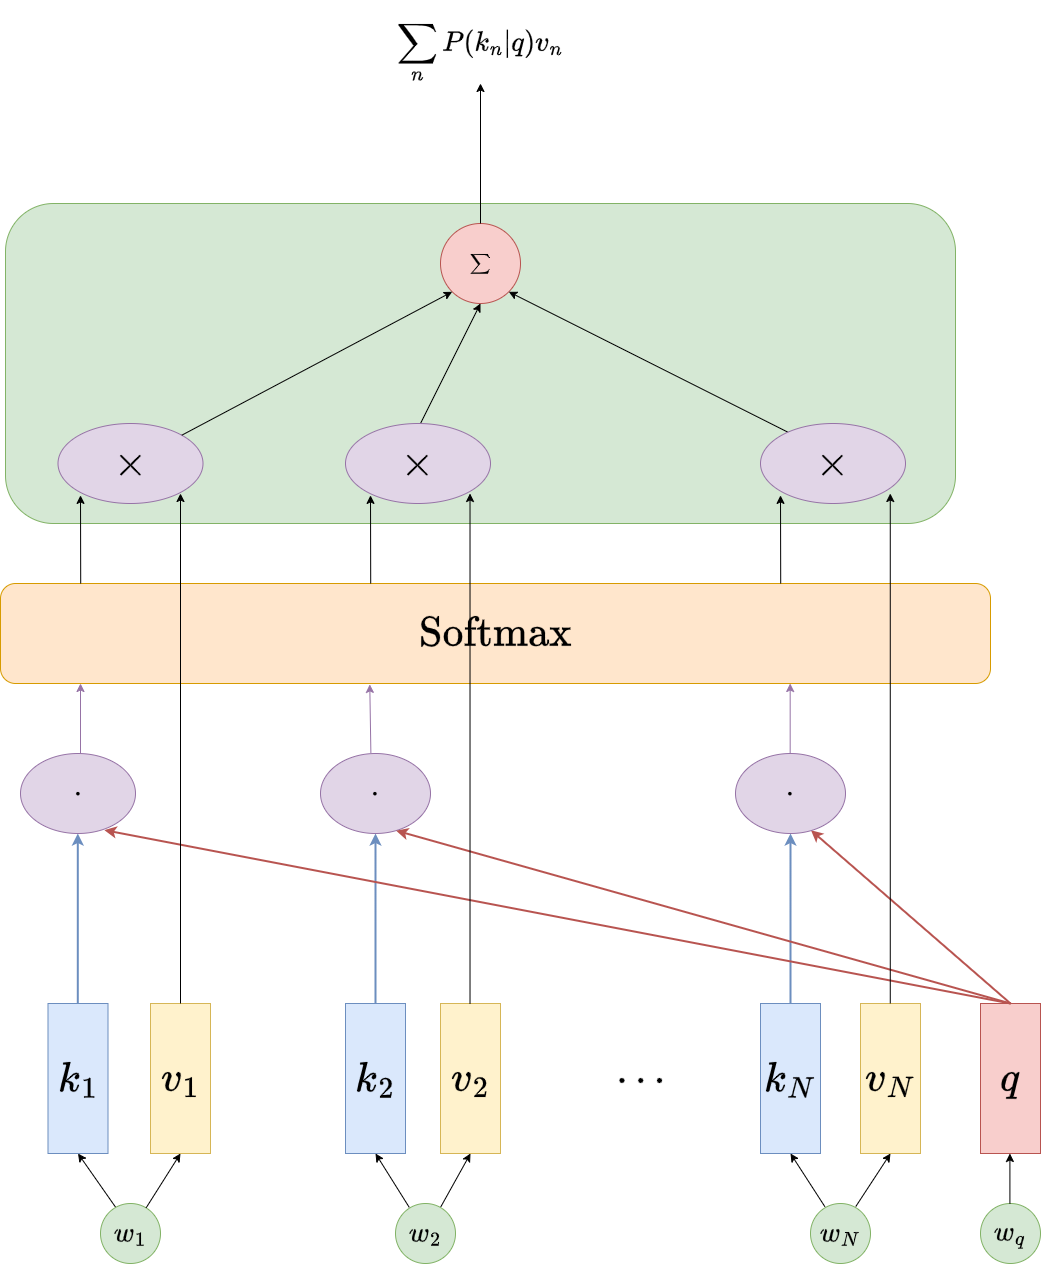
\includegraphics[width=0.45\linewidth]{images/transformers_images/elementwise_attention.png}
            \caption*{The end result is messy, which is why we tend to go for the matrix-based notation.}
        \end{figure}

        


        


        


    \pagebreak
        
    \subsection{RNNs: a review}

        Our new \vocab{attention mechanism}, is a powerful tool for language processing. We'll develop this in three stages:

        \begin{itemize}
            \item Reviewing our old language model: the \gren{recurrent neural network (RNN)}.
            
            \item Improving on the RNN model with \purp{attention}.

            \item Moving past RNNs, to create an \orgg{attention-only} model.
                \note{\href{https://arxiv.org/abs/1706.03762}{Attention is All You Need}, one might say.}
        \end{itemize}

        First: what exactly does a "language model" do? Language stuff, I presume. 

        \begin{itemize}
            \item But we need to be more specific, if we want to solve a real problem.\\
        \end{itemize}

        \begin{definition}
            A basic \vocab{language model} follows the \orgg{predictive text} problem:
            
            \begin{itemize}
                \item You predict the \gren{next word} in a sentence, given \purp{previous words}.
            \end{itemize}
        \end{definition}

        \begin{itemize}
            \item \miniex This is similar to a phone's "autocomplete", which suggests a completed sentence, based on a partial text.
        \end{itemize}

        Previously, we used RNNs to handle this problem. Let's review the basic structure of an RNN:
            \note{If you want to review a little more in-depth, revisit chapter 10. For language stuff in particular, review 10.4.}

        \begin{figure}[H]
            \centering
            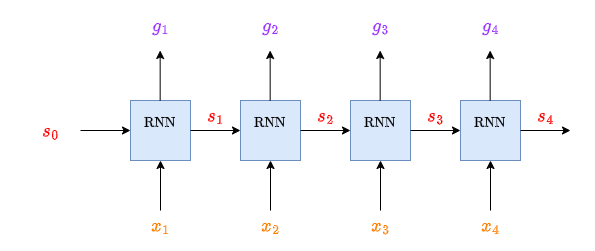
\includegraphics[width=100mm]{images/rnn_images/rnn_simple_g_notation.png}
            \caption*{At each timestep $t$, our model takes in an \orgg{input} $x_t$, saves information in \redd{state} $s_t$, and \purp{outputs} a value $g_t$.}
        \end{figure}

        \begin{concept}
            In a \vocab{language model RNN}, each input $x_t$ is a \orgg{token}, representing one part of the text.

            \begin{itemize}
                \item Tokens which come later in a \gren{sentence}, are presented to the RNN later in \purp{time}.
            \end{itemize}
        \end{concept}

        These inputs are "remembered" using our state, $s_t$.\\

        \begin{concept}
            In a \vocab{language model RNN}, our \redd{state $s_t$} stores information about the \purp{inputs} we've received before: all of the \orgg{context} in our sentence.

            \begin{itemize}
                \item Our RNN uses this context to \purp{predict} our next token.
            \end{itemize}
        \end{concept}
            

        \begin{figure}[H]
            \centering
            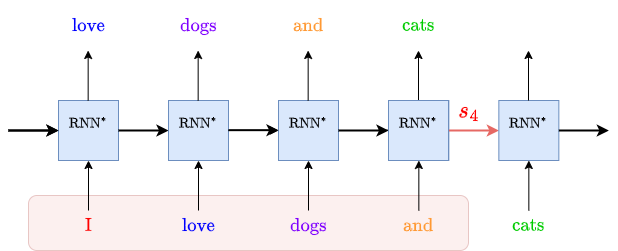
\includegraphics[width=0.7\linewidth]{images/transformers_images/rnn_state_memory.png}
            \caption*{In a good RNN, we hope that state $s_4$ would contain info about the entire sentence portion that comes before: "I like dogs and".}
        \end{figure}

        Technically, we should turn our words into vector embeddings first. We'll skip that step, for visual simplicity.
            \note{All we would need is to turn each word into a \purp{value vector}.}



    \phantom{}

    \subsection{RNNs: Encoding}

        This property of RNNs is interesting: \redd{$s_t$} is designed to \purp{encode} information about the prior inputs.

        \begin{itemize}
            \item This might remind of our \vocab{autoencoders} from an earlier chapter.\\
        \end{itemize}

        \begin{concept}
            Our RNN can be thought of as an \vocab{encoder}: it compresses our input $x$ into a more \gren{compressed} representation.

            \begin{itemize}
                \item This information is represented in the \redd{state $s_T$}.
            \end{itemize}

            In particular, because RNNs process \purp{sequential} data (like text), it can be used to \orgg{encode sequential information}.
        \end{concept}

        We've created a new type of encoder! 

        \begin{itemize}
            \item Unlike a fully-connected NN (our previous style of encoder), this handles information \gren{over time}.
        \end{itemize}

        We could take an entire sentence, and \purp{encode} its useful information with an RNN.

        \begin{figure}[H]
            \centering
            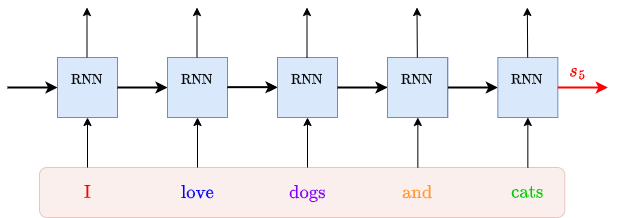
\includegraphics[width=0.7\linewidth]{images/transformers_images/rnn_encoder.png}
            \caption*{After we've fed in all of our inputs, we hope that $s_5$ encodes the meaning of the sentence: "I love dogs and cats".}
        \end{figure}

        The \redd{encoding $s_5$} is what we're interested in. We'll omit the other outputs, for simplicity.

        \begin{figure}[H]
            \centering
            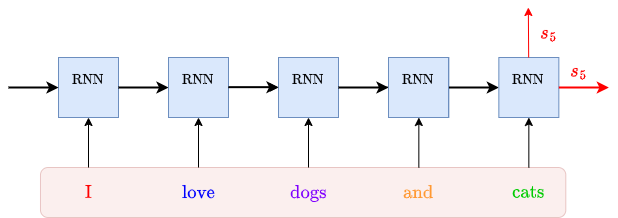
\includegraphics[width=0.7\linewidth]{images/transformers_images/rnn_encoder_outputless.png}
            \caption*{We don't know the full meaning of the sentence until we finish. So, we'll just focus on the state after seeing \purp{every input}.}
        \end{figure}

        Notice that we \orgg{changed our output function}: $s_5$ is the output for the $\nth{5}$ timestep, $g_5$!\\

        \begin{definition}
            Our \vocab{encoder RNN} returns its \redd{state $s_t$} as its \brow{output $g_t$}.

            \begin{itemize}
                \item The state is the \purp{compressed representation} of the input $x$.

                \item For an encoder, that's the \gren{most important information}: hence, we provide it as output.
            \end{itemize}

            \begin{equation*}
                g_t = s_t
            \end{equation*}
        \end{definition}



    \phantom{}

    \subsection{RNNs: Decoding}

        Following this train of logic, we can create an \vocab{autoencoder}: we just have to \purp{decode} our state with a second RNN.

        \begin{itemize}
            \item We'll start from our compressed state, $s_5$.
        \end{itemize}

        \begin{figure}[H]
            \centering
            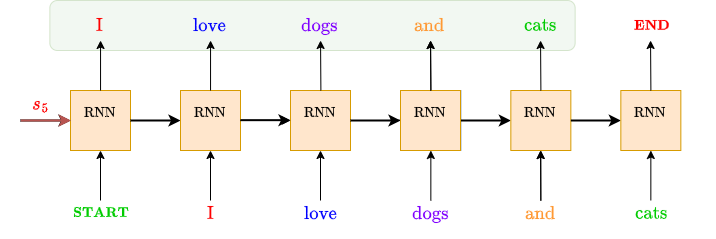
\includegraphics[width=100mm]{images/transformers_images/rnn_decoder.png}
            \caption*{Now, this looks similar to our text prediction problem from before.}
        \end{figure}

        Similar to the text prediction problem, we'll feed in the correct answers as an input, \textit{after} our model predicts it.
            \note{If we don't have a "correct" answer, we can just use our model's previous output as the input.}

        With any luck, we'll get the above, and the decoder can reproduce the original input, based on the state.\\

        \begin{definition}
            Our \vocab{decoder RNN} starts with \redd{state $s_T$}, representing the sentence received by the \gren{encoder RNN}.

            \begin{itemize}
                \item The goal is to sequentially \purp{reproduce} the sentence that created $s_T$.
            \end{itemize}

            This model works similar to the text prediction problem: it receives the \gren{correct input} one timestep after it predicts it.
        \end{definition}

        And with this, we have a complete autoencoder.

    \phantom{}

    \subsection{RNNs: Translation}

        This autoencoder system is cool, but maybe a little basic: we've already seen autoencoders before.

        \begin{itemize}
            \item Instead, we'll try a different task: \purp{translation!}
        \end{itemize}

        Here's our general idea:

        \begin{itemize}
            \item We can \purp{encode} text in one language, into a compressed format.

            \item Then, we \gren{decode} that text, in a different language.
        \end{itemize}

        The meaning is preserved, with the grammar and vocab shifted to suit the language.\\

        \begin{definition}
            In the \vocab{RNN translation task}, we use an encoder-decoder system to convert text \orgg{between languages}.

            \begin{itemize}
                \item \vocab{Encoder}: We input our target text, and it outputs as \redd{$s_T$}: this should represent the \purp{meaning} of the sentence.

                \item \vocab{Decoder}: We input the embedding \redd{$s_T$}, and it outputs a \purp{translation} of our text into \gren{another language}.
            \end{itemize}
            
        \end{definition}


        \miniex We'll convert text from japanese to english. Our example text: "kore wa yokunai".

        \begin{itemize}
            \item First, we encode our \purp{japanese} into a \redd{state}.

            \begin{figure}[H]
                \centering
                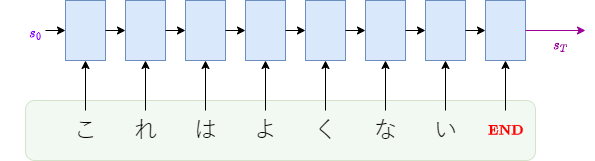
\includegraphics[width=100mm]{images/transformers_images/rnn_translate_encode.png}
                \caption*{Our RNN is trained to understand japanese grammar and vocabulary.}
            \end{figure}

            \item Then, we reverse this: turning our \redd{state} into an \gren{english} sentence.

            \begin{figure}[H]
                \centering
                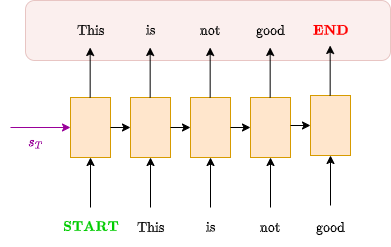
\includegraphics[width=70mm]{images/transformers_images/rnn_translate_decode.png}
                \caption*{Our RNN can "decode" the information in the state $s_T$, and turn it into english.}
            \end{figure}
        \end{itemize}

        All together, we have a system we can use to translate whatever sentence we'd like.

        \begin{figure}[H]
            \centering
            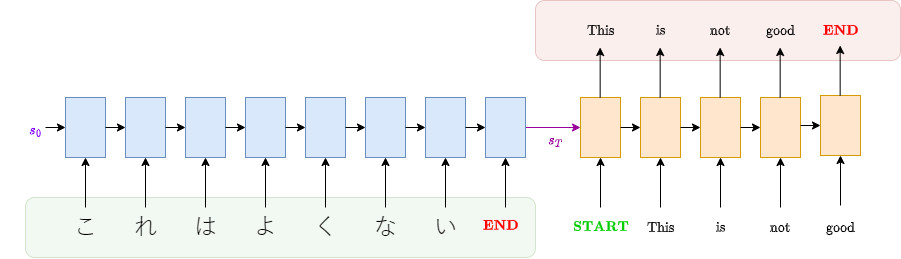
\includegraphics[width=\linewidth]{images/transformers_images/rnn_translate.png}
            \caption*{Our japanese prompt is shown in green, and our english response is shown in red.}
        \end{figure}

        
        
    \redd{CHAPTER IS INCOMPLETE}


\pagebreak


\iffalse


    \phantom{}


        


    \subsection{Attention-based RNNs}

        %Attention go brrr

        



\section{Old Materials}

%%%%%%%%%%%%%%%%%%%%%%%%%%%%%%%%%%%%%%%%%%%%%%%%%%%%%%%%%%%%%%%%%%%%%%%%%%%%%
\section{Attention}
\label{sec:attention}

% - query, key, value
%
%   - dict storing foods, with keys pizza, apple, sandwich, donut, chili, burito, sushi, hamburger, ...
%   - goal is to look up a food based on something more general, e.g., "convenient" or "spicy"
%   - need way to learn unstructured relationships.
%   - query q = column vector, K = matrix of keys
%   - attention distribution alpha = softmax(q^T K)
%   - attention(q,K,v) = softmax(q^T K) . v
%   - let d_k be the dimension of each key, then to keep gradients well-sized, do
%     attention(q,K,v) = softmax(q^T K / sqrt{d_k}) . v


%%%%%%%%%%%%%%%%%%%%%%%%%%%%%%%%%%%%%%%%
\subsection{Towards language models with attention}
% seq2seq with RNNs


% problem with RNNs
%
% - need for complex patterns: towards multi-headed attention
%
%   - sentence that needs a long window
%     Unlike the other white ducks in the pond, its feathers were _____
%     Just like the other white ducks in the pond, its feathers were _____
%
%   - Not all words are important
%     Judy needed to figure out how many pumpkins to buy for the party.
%     Since twenty guests were coming and three could share one pumpkin, she decided to buy ______
%
%   - The important words may appear anywhere in the sentence
%     Weather forcasts have clearly gotten much ______ since the since the game started 
%     allowing magic users to abruptly change seasons in the fantasy world
This can work pretty well for short prompts.  The challenge comes when the input sequence is long, because all the information about the prompt must be encoded in the final state of the encoder RNN.  And the state of an RNN typically becomes increasingly uncorrelated with a given input the further away it is in time.  For language translation, this is a pressing problem when the two languages have different grammar.  In Japanese, the sentiment of a sentence can be completely changed by the suffix added to the verb at the very end of the sentence.  This means that to accurately translate Japanese to English, the encoder RNN in our example needs to know both the initial and final Japanese words.  But the RNN will perform increasingly poorly as the input sentence gets longer.

% seq2seq with attention
Alternatively, an attention mechanism can be employed.  Conceptually, what we want is for the current state of the decoder RNN to be able to pay attention to a specific state vector of the encoder RNN, instead of just looking at the encoder RNN's final state.  For example, after outputting the word ``is,'' the decoder RNN in our Japanese translation scenario would want to know most about encoder RNN's state specifically at the word ``nai'' in the input, since that would generate the following English word in the output, ``not.''  We can accomplish this by employing the state of the encoder RNN as being both the keys and values, and letting the current state of the decoder RNN be the query, using this conceptual structure:
\begin{center}
\includegraphics[width=4.615in]{figures/seq2seq-with-attention.png}
\end{center}
This is the conceptual structure of a seq2seq RNN with attention.  The top vector at the output of the softmax is the attention output, and this output is then used together with the decoder RNN's current state to produce the next output word.

% patterns not based on spatial (CNN) or temporal (RNN) locality
This usage of an attention mechanism bestows the RNNs with a kind of long-term memory, since generation of the output word can now utilize information from any word in the input sequence that is used to generate the attention output.  There are more sophisticated structures than the simple conceptual example given above.  For instance, the keys and values could use different vector embeddings, and an embedding could be applied to the values used to generate the attention output.  How the decoder employs the attention output to generate the next word can also be sophisticated.  And attention mechanisms are valuable not just for sequential data, but also for spatial data such as images.  Note that all of these embeddings and generation processes are generally neural networks that are trainable using back-propagation.  Actually training these embeddings can be difficult in practice, because of the large number of degrees of freedom, particularly as the number of keys and values grows.  But the main point to take away from this discussion is that attention mechanisms allows modeling of a far richer set of patterns than the temporally local RNN models, or even the spatially local CNN models, when applied to images.


%%%%%%%%%%%%%%%%%%%%%%%%%%%%%%%%%%%%%%%%%%%%%%%%%%%%%%%%%%%%%%%%%%%%%%%%%%%%%
\section{Transformers}
\label{sec:transformers}

Looking at the structure of the seq2seq RNN with attention, you might wonder why the RNN is needed, given the attention mechanism.  In fact, the RNN structure is not needed, and can be replaced with a suitable combination of attention mechanisms, using a structure known as a ``transformer.''  At the heart of the transformer is the idea of self-attention.

% self attention
%  - key, query, value embedding
Self-attention is an attention mechanism where the keys, values, and queries are all generated from the same input.  The idea is that for some input $x$, we generate a key $\kappa = (W^k)^T x$ using a weight matrix $W^k$, a value $v = (W^v)^T x$ with weight matrix $W^v$, and a query using $(W^q)^T x$.  The attention mechanism then uses the attention function $\kappa^T q$ to determine which inputs are most relevant to a given $q$.  In the context of our language translation example, this means that attention is used to determine which tokens (moving forward, let us think more generally, focusing on tokens instead of words) are most strongly related to each other.  The attention output is then used to produce an output token.  The neural network structure looks like this:
\begin{center}
\includegraphics[width=2.615in]{figures/transformer-self-attention.png}
\end{center}
This diagram shows the middle input token generating a query that is then combined with the keys computed with all the other tokens to generate the attention weights via a softmax.  The output of the softmax is then combined with values computed from the other tokens, to generate the attention output corresponding to the middle input token.  Repeating this for each input token then generates the output.

%  - output size same as input
%  - position encoding
%  - masking
Note that the size of the output is the same as the size of the input.  Also, observe that there is no apparent notion of ordering of the input words in the depicted structure.  Positional information can be added by encoding a number for token (giving say, the token's position relative to the start of the sequence) into the vector embedding of each token.  And note that a given query need not pay attention to all other tokens in the input; in this example, the token used for the query is not used for a key or value.

% masking
More generally, a {\em mask} may be applied to limit which tokens are used in the attention computation.  For example, one common mask limits the attention computation to tokens that occur previously in time to the one being used for the query.  This prevents the attention mechanism from ``looking ahead'' in scenarios where the transformer is being used to generate one token at a time.

% difference from RNN
This single stage of self-attention is the principal component of a {\em transformer block}, and it is meaningfully different from an RNN: the transformer does not have a recurrent structure.  Thus, back-propagation-though-time does not need to be used, and the vanishing gradients problem of RNN's does not arise in the same way.  Moreover, all input tokens can be processed at once, instead of one at a time.  This means a transformer can be much faster to train than a comparable RNN: instead of requiring a number of training steps that grows linearly with the size of the input, the transformer can be trained in a single step, as long as sufficient computational resources are available for the parallel processing.

% multi-headed attention
Each self-attention stage is trained to have key, value, and query embeddings that lead it to pay specific attention to some particular feature of the input.  We generally want to pay attention to many different kinds of features in the input; for example, in translation one feature might be be the verbs, and another might be objects or subjects.  A transformer utilizes multiple instances of self-attention, each known as an ``attention head,'' to allow combination of attention paid to many different features.  

%%%%%%%%%%%%%%%%%%%%%%%%%%%%%%%%%%%%%%%%
\subsection{Formal definition of a transformer}

% formal definition
%
% Mathematical summary, following John Thickstun, but rewritten in 6.390 standard notation
% 6.390 conventions are that
% data input = d x n (each column is a data vector)
% superscript x^{(i)} indicates sample number
% NN output is W^T X
% need to include heads
%
% layer norm?
% residual connections?
%
A transformer is the composition of a number of transformer blocks, each of which has multiple heads.  Rather than depicting this graphically, it is worth returning to the beauty of the underlying equations\footnote{The presentation here follows the lovely notes by John Thickstun, rewritten into the standard notational conventions of 6.390.}.  Please note that in the following, we take samples $x^{(i)}$ to be colum vectors, i.e. $\R^{d \times 1}$.
%
Formally, a transformer block is a parameterized function $f_\theta$ that maps $\R^{d\times n}\rightarrow R^{d\times n}$, where $n$ is the number of tokens, $d$ is the dimension of each token, and $\theta$ are the model parameters.  If $x\in \R^{d\times n}$ then $f_\theta(x) = z$ where queries, keys, and values are embedded via encoding matrices:
\begin{eqnarray}
  Q^{(h)}(x^{(i)}) &=& (W_{h,q})^T x^{(i)}
\\
  K^{(h)}(x^{(i)}) &=& (W_{h,k})^T x^{(i)}
\\
  V^{(h)}(x^{(i)}) &=& (W_{h,v})^T x^{(i)}
\end{eqnarray}
and $W_{h,q}, W_{h,k}, W_{h,v} \in \R^{d\times d_k}$, where $d_k$ is the size of the key space, $i \in \{1,\cdots,n\}$ is an integer index over tokens, and $h \in \{1,\cdots,H\}$ is an index over ``transformer heads.''  The attention weights $\alpha^{(h)}_{ij}$ for head $h$, query $i$ and key $j$ are then given by
\begin{eqnarray}
  \alpha^{(h)}_{ij} = \text{softmax}_j \left( \frac{Q^{(h)}(x^{(i)})^T K^{(h)}(x^{(j)})}{\sqrt{d_k}}  \right)
\,.
\label{eq:xfm_softmax}
\end{eqnarray}
Here, $\text{softmax}_j$ is a softmax over the $d_k$-dimensional vector indexed by $j$, so in Eq.~\ref{eq:xfm_softmax} this means a softmax computed over keys.  In this equation, the normalization by $\sqrt{d_k}$ is done to reduce the magnitude of the dot product, which would otherwise grow undesirably large with increasing $d_k$.

The un-normalized attention outputs are a weighted sum over the attention outputs for each head,
\begin{eqnarray}
  {u'}^{(i)} = \sum_{h=1}^H W^T_{h,c} \sum_{j=1}^{n} \alpha^{(h)}_{ij} V^{(h)}(x^{(j)})
\,,
\end{eqnarray}
where $W_{h,c} \in \R^{d_k\times d}$.  This is standardized and combined with $x^{(i)}$ using a $\text{LayerNorm}$ function (defined below) to become
\begin{eqnarray}
  {u}^{(i)} = \text{LayerNorm}\left(  x^{(i)} + {u'}^{(i)}; \gamma_1, \beta_1  \right)
\end{eqnarray}
with parameters $\gamma_1, \beta_1 \in \R^{d}$.  The un-normalized transformer block output ${z'}^{(i)}$ is then given by
\begin{eqnarray}
  {z'}^{(i)} = W_2^T \text{ReLU}\left( W_1^T u^{(i)} \right)
\end{eqnarray}
with weights $W_1\in \R^{d\times m}$ and $W_2\in \R^{m\times d}$.  This is then standardized and combined with $u^{(i)}$ to give the final output $z^{(i)}$:
\begin{eqnarray}
  {z}^{(i)} = \text{LayerNorm}\left(  u^{(i)} + {z'}^{(i)}; \gamma_2, \beta_2  \right)
\,,
\end{eqnarray}
with parameters $\gamma_2, \beta_2 \in \R^{d}$.  These vectors are then assembled (e.g., through parallel computation) to produce $z\in \R^{n\times d}$.

The $\text{LayerNorm}$ function transforms a $d$-dimensional input $z$ with parameters $\gamma, \beta \in \R^d$ into
\begin{eqnarray}
  \text{LayerNorm}(z; \gamma, \beta) = \gamma \frac{z-\mu_z}{\sigma_z} + \beta
\,,
\end{eqnarray}
where $\mu_z$ is the mean and $\sigma_z$ the standard deviation of $z$:
\begin{eqnarray}
  \mu_z &=& \frac{1}{d} \sum_{i=1}^d z_i
  \\
  \sigma_z &=& \sqrt{ \frac{1}{d} \sum_{i=1}^d (z_i-\mu_z)^2 }
\,.
\end{eqnarray}
Layer normalization is done to improve convergence stability during training.

The model parameters $\theta$ comprise the weight matrices $W_{h,q}, W_{h,k}, W_{h,v}, W_{h,c}, W_1, W_2$ and the $\text{LayerNorm}$ parameters $\gamma_1, \gamma_2, \beta_1, \beta_2$.  A {\em transformer} is the composition of $L$ transformer blocks, each with its own parameters:
\begin{eqnarray}
  f_{\theta_L} \circ  \cdots \circ f_{\theta_2} \circ f_{\theta_1}(x) \in R^{d\times n}
\,.
\end{eqnarray}
The hyperparameters of this model are $d, d_k, m, H,$ and $L$, where typically $d=512$, $d_k = 64$, $m=2048$, $H=8$, and $L\ge 6$.


%%%%%%%%%%%%%%%%%%%%%%%%%%%%%%%%%%%%%%%%
\subsection{Variations and training}

Many variants on this transformer structure exist.  For example, the $\text{LayerNorm}$ may be moved to other stages of the neural network.  Or a more sophisticated attention function may be employed instead of the simple dot product used in Eq.~\ref{eq:xfm_softmax}.  Transformers may also be used in pairs, for example, one to process the input and a separate one to generate the output given the transformed input.  Self-attention may also be replaced with cross-attention, where some input data are used to generate queries and other input data generate keys and values.  Positional encoding and masking are also common, though they are left implicit in the above equations for simplicity.

How are transformers trained?  The number of parameters in $\theta$ can be very large; modern transformer models like GPT4 have tens of billions of parameters or more.  A great deal of data is thus necessary to train such models, else the models may simply overfit small datasets.

Training large transformer models is thus generally done in two stages.  A first ``pre-training'' stage employs a very large dataset to train the model to extract patterns.  This is done with unsupervised (or self-supervised) learning and unlabelled data.  For example, the well-known BERT model was pre-trained using sentences with words masked off.  The model was trained to predict the masked words.  BERT was also trained on sequences of sentences, where the model was trained to predict whether two sentences are likely to be contextually close together or not.  The pre-training stage is generally very expensive.

The second ``fine-tuning'' stage trains the model for a specific task, such as classification or question answering.  This training stage can be relatively inexpensive, but it generally requires labeled data.

\fi

